\chapter{Играта 15}

\begin{figure}[H]
  \centering
  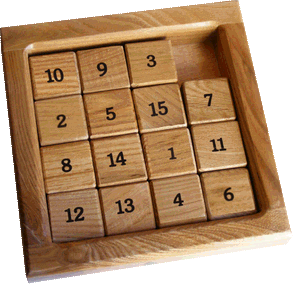
\includegraphics[width=1.0\linewidth,height=0.5\linewidth]{fig060001.png}
  \caption{„Играта 15“ \\ http://www.murderousmaths.co.uk/games/loyd/15 puzzle wood.gif}
\label{fig060001}
\end{figure}

„Играта 15“ (Фиг. \ref{fig060001}) е детски пъзел от групата игри „пътешествие по граф“. Игралното поле е оформено в 4x4 клетки, като в него са поместени 15 плочки. Плочките са номерирани и шестнадесетата позиция е празна. Празната позиция служи като буфер в който могат да се местят съседните плочки. С помощта на буферната клетка, играта се разбърква и целта е плочките да бъдат подредени според началната номерация. 

Това е детска игра, подреждането на която не е особено трудно и сложност създава единствено последния ред в пъзела. Относително простичката организация на играта я прави идеална за реализация като App Inventor приложение. С помощта само на 16 бутона може да се изгради целият нужен интерфейс. Изработката започва със създаването на нов проект (Фиг. \ref{fig060002}).

\begin{figure}[H]
  \centering
  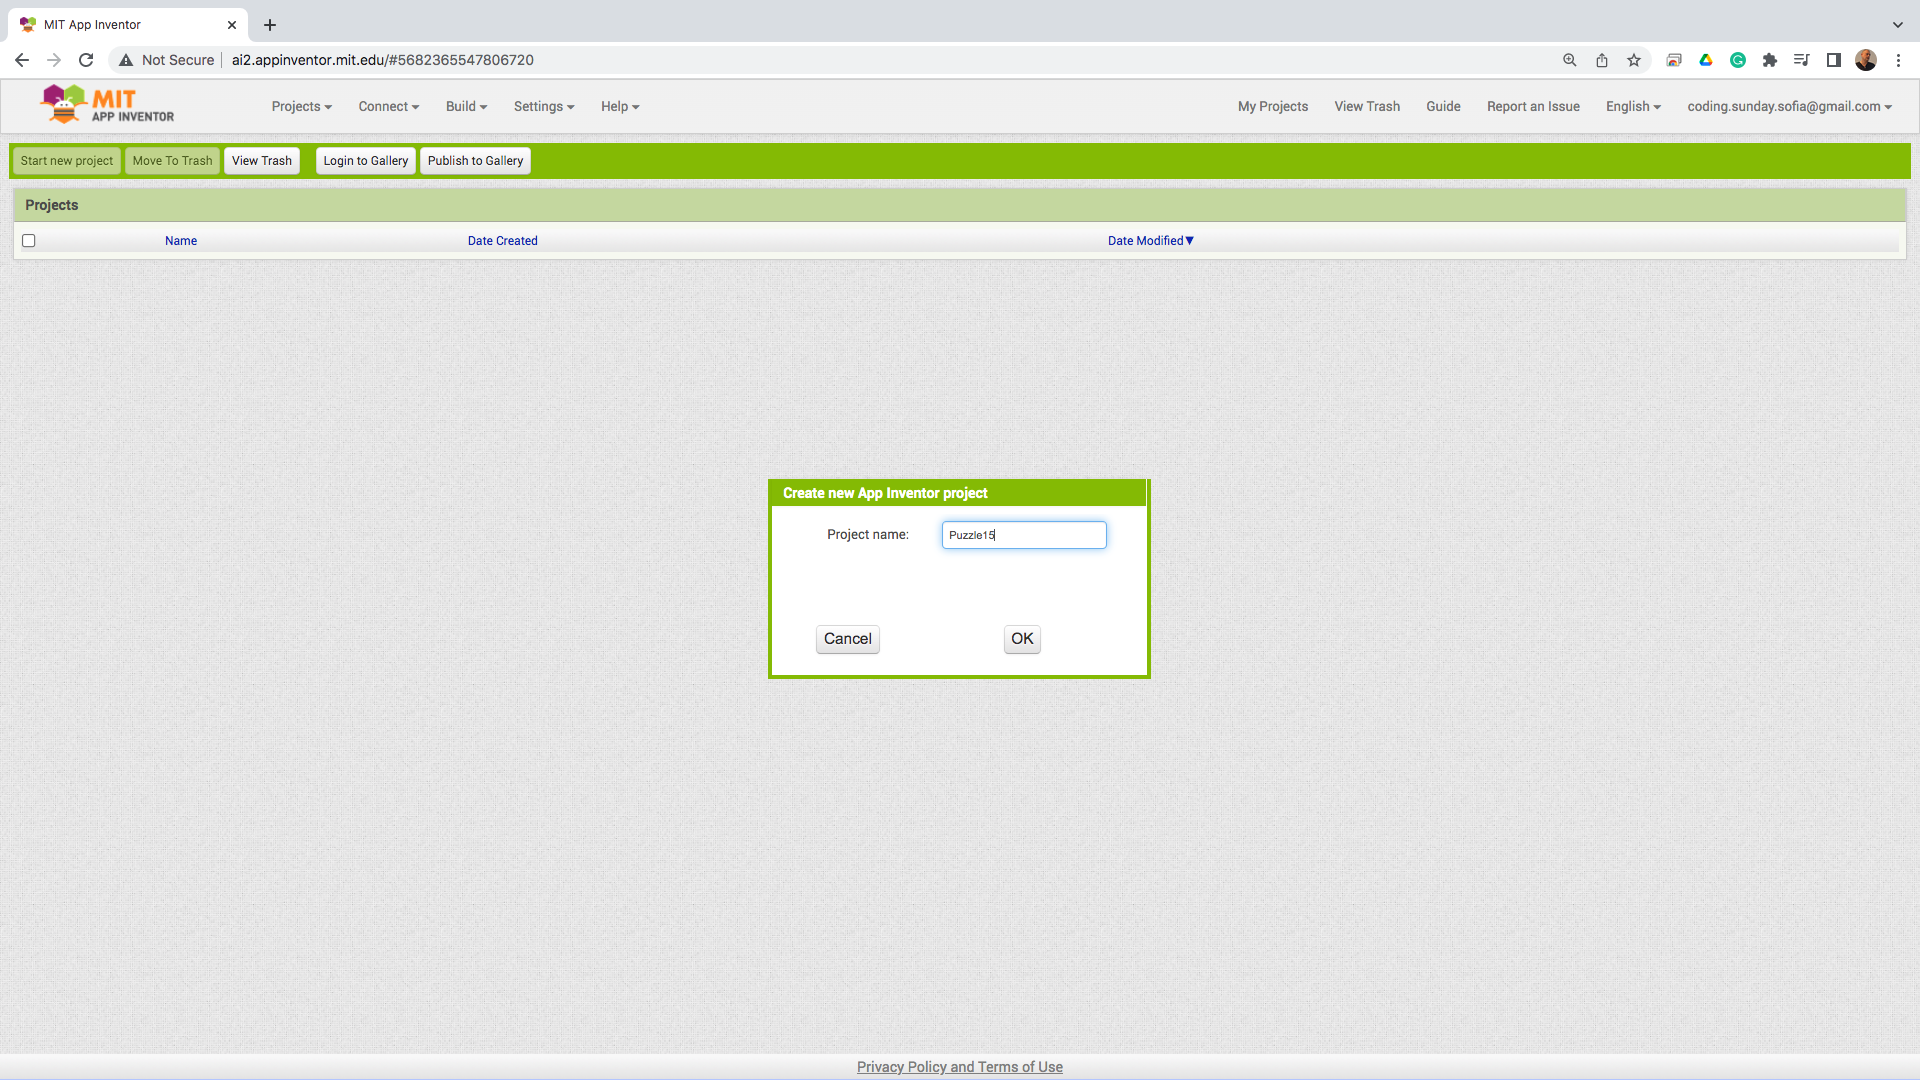
\includegraphics[width=1.0\linewidth,height=0.5\linewidth]{fig060002.png}
  \caption{Стартиране на нов проект за „Играта 15“}
\label{fig060002}
\end{figure}

Тъй като ще се използват 15 номерирани бутона и един без номерация, то най-удачно е те да бъдат организирани с мениджър на разположението от тип таблица, с 4 реда и 4 колони (Фиг. \ref{fig060003}).

\begin{figure}[H]
  \centering
  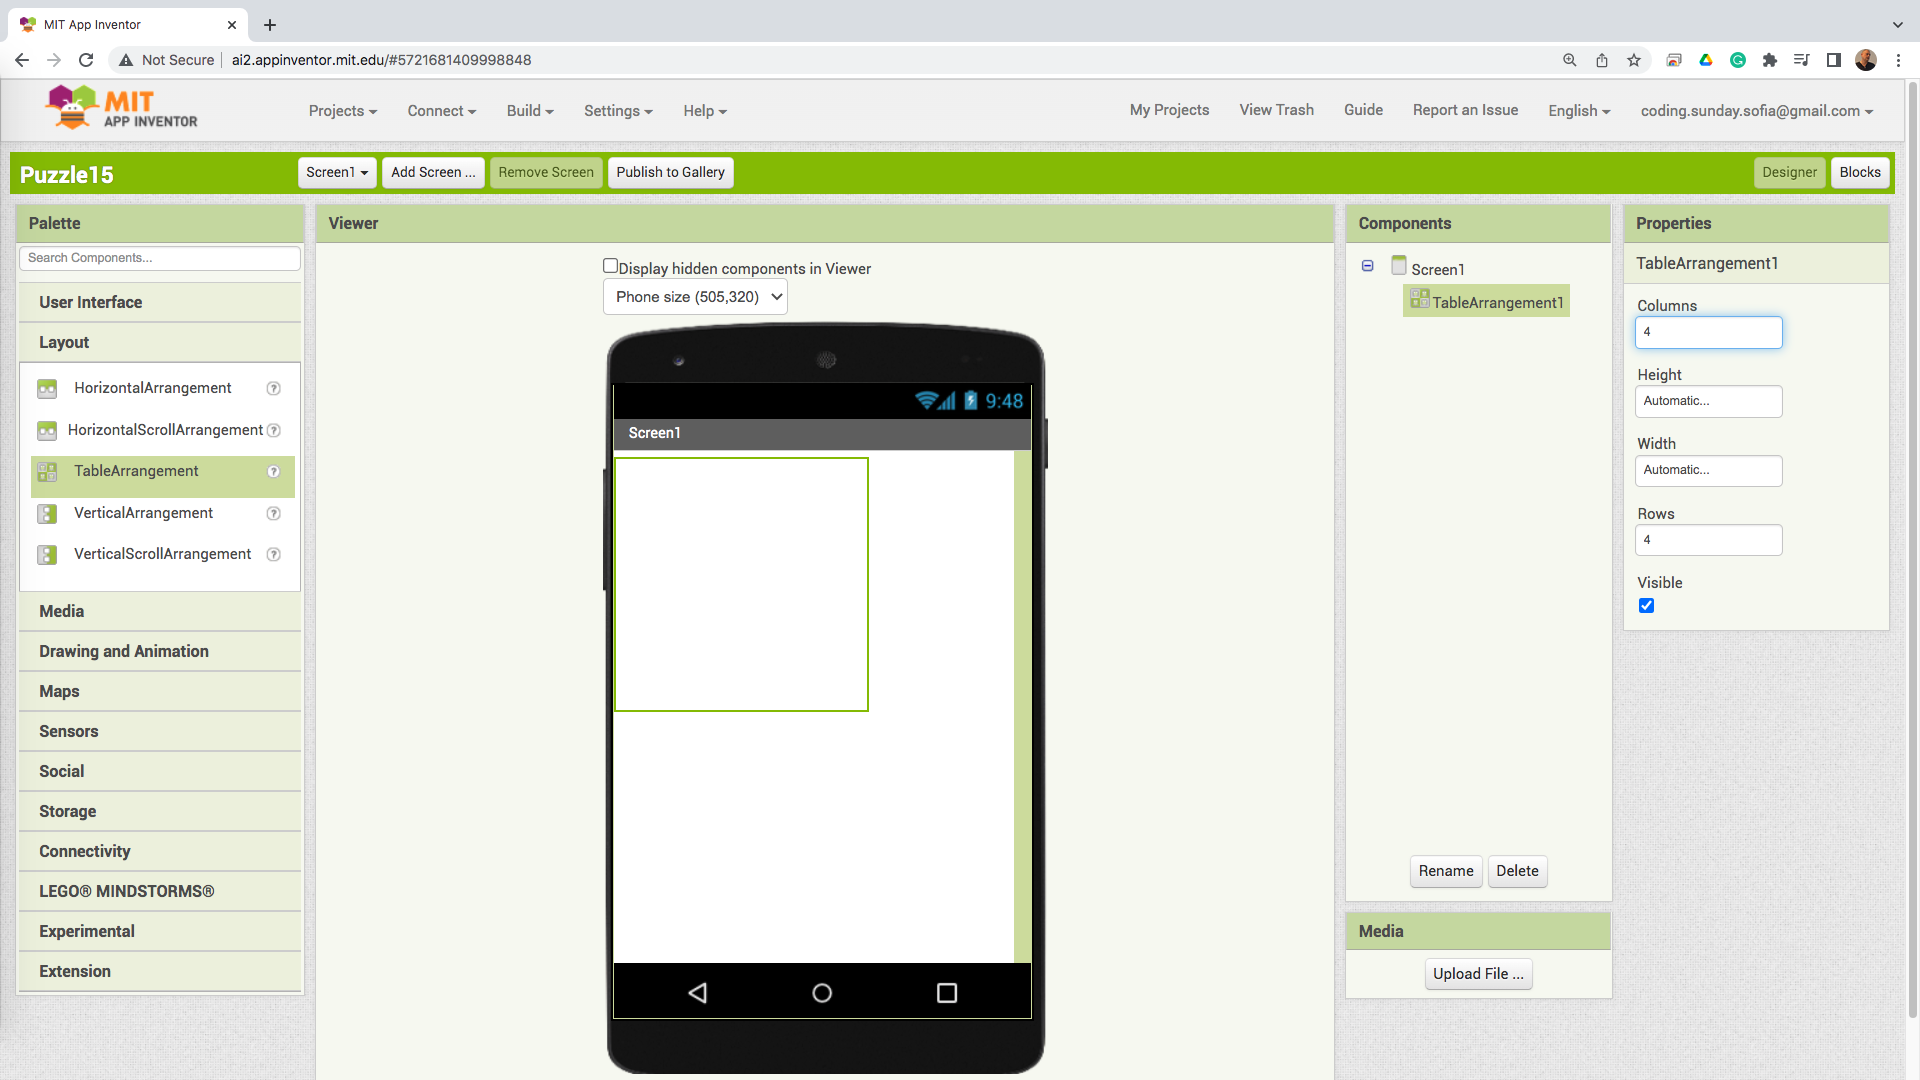
\includegraphics[width=1.0\linewidth,height=0.5\linewidth]{fig060003.png}
  \caption{Мениджър на съдържанието с 4x4 клетки}
\label{fig060003}
\end{figure}

Следва поставяне на 16 бутона (Фиг. \ref{fig060004}), като нечетните числа се оцветяват в червено, а четните числа в синьо. Оцветяването подсилва визуалния ефект на играта. Шестнадесетият бутон вместо надпис има два празни интервала, така че ширината му да съвпада с ширината на другите бутони. Без допълнителни настройки, ширината на бутоните се определя от броя символи в надписите им. 

\begin{figure}[H]
  \centering
  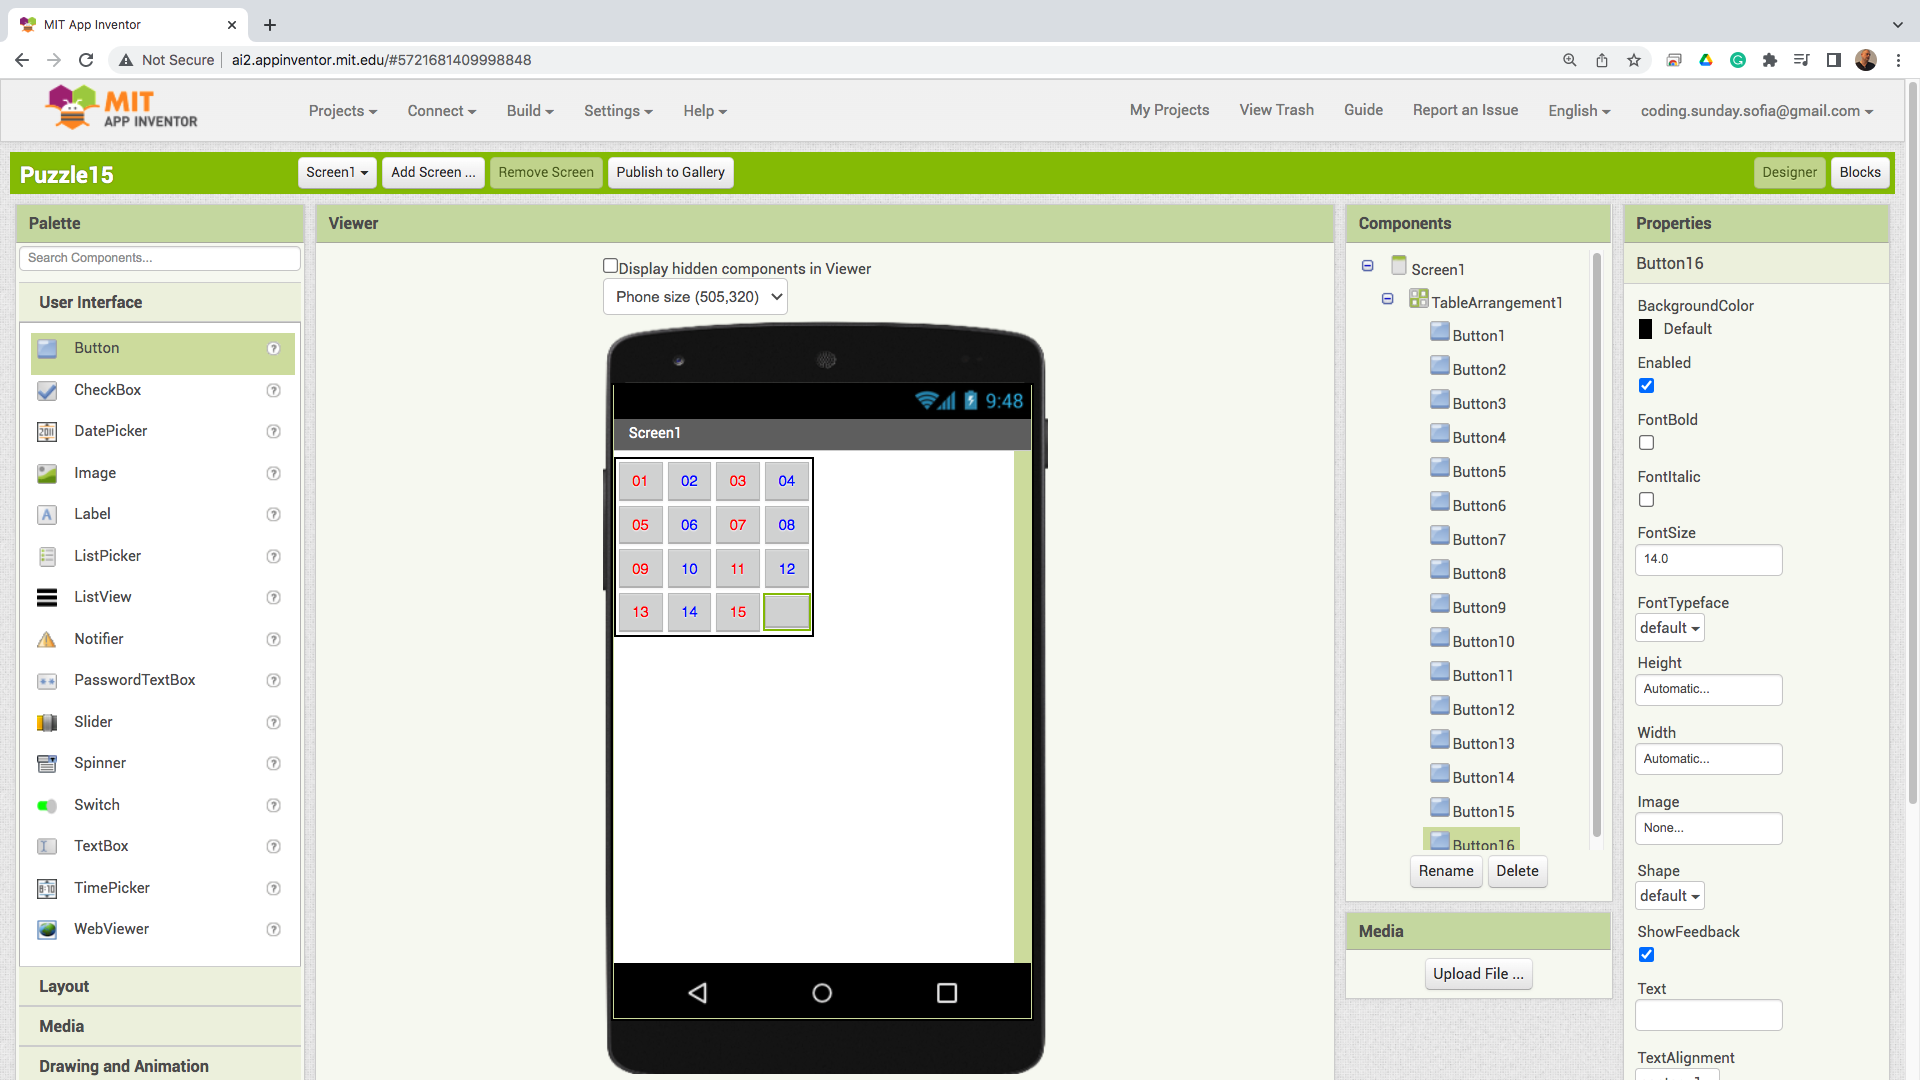
\includegraphics[width=1.0\linewidth,height=0.5\linewidth]{fig060004.png}
  \caption{Поставяне на 16 бутона}
\label{fig060004}
\end{figure}

Възможно е да се разменят самите бутони, когато се натисне бутон в съседство на празната клетка, но значително по-лесно е да се разменят надписите и цветовете на бутоните, а самите бутони да остават винаги на първоначалните си места. Натискането на бутона ще се прихваща в общо събитие за всички бутони, но след натискането трябва да се определи дали в съседство е празната клетка. Най-елегантно съседството може да бъде установено, ако структура от тип речник съдържа всички бутони като ключове (Фиг. \ref{fig060005}), а като стойности списъчни структури със съседите.

\begin{figure}[H]
  \centering
  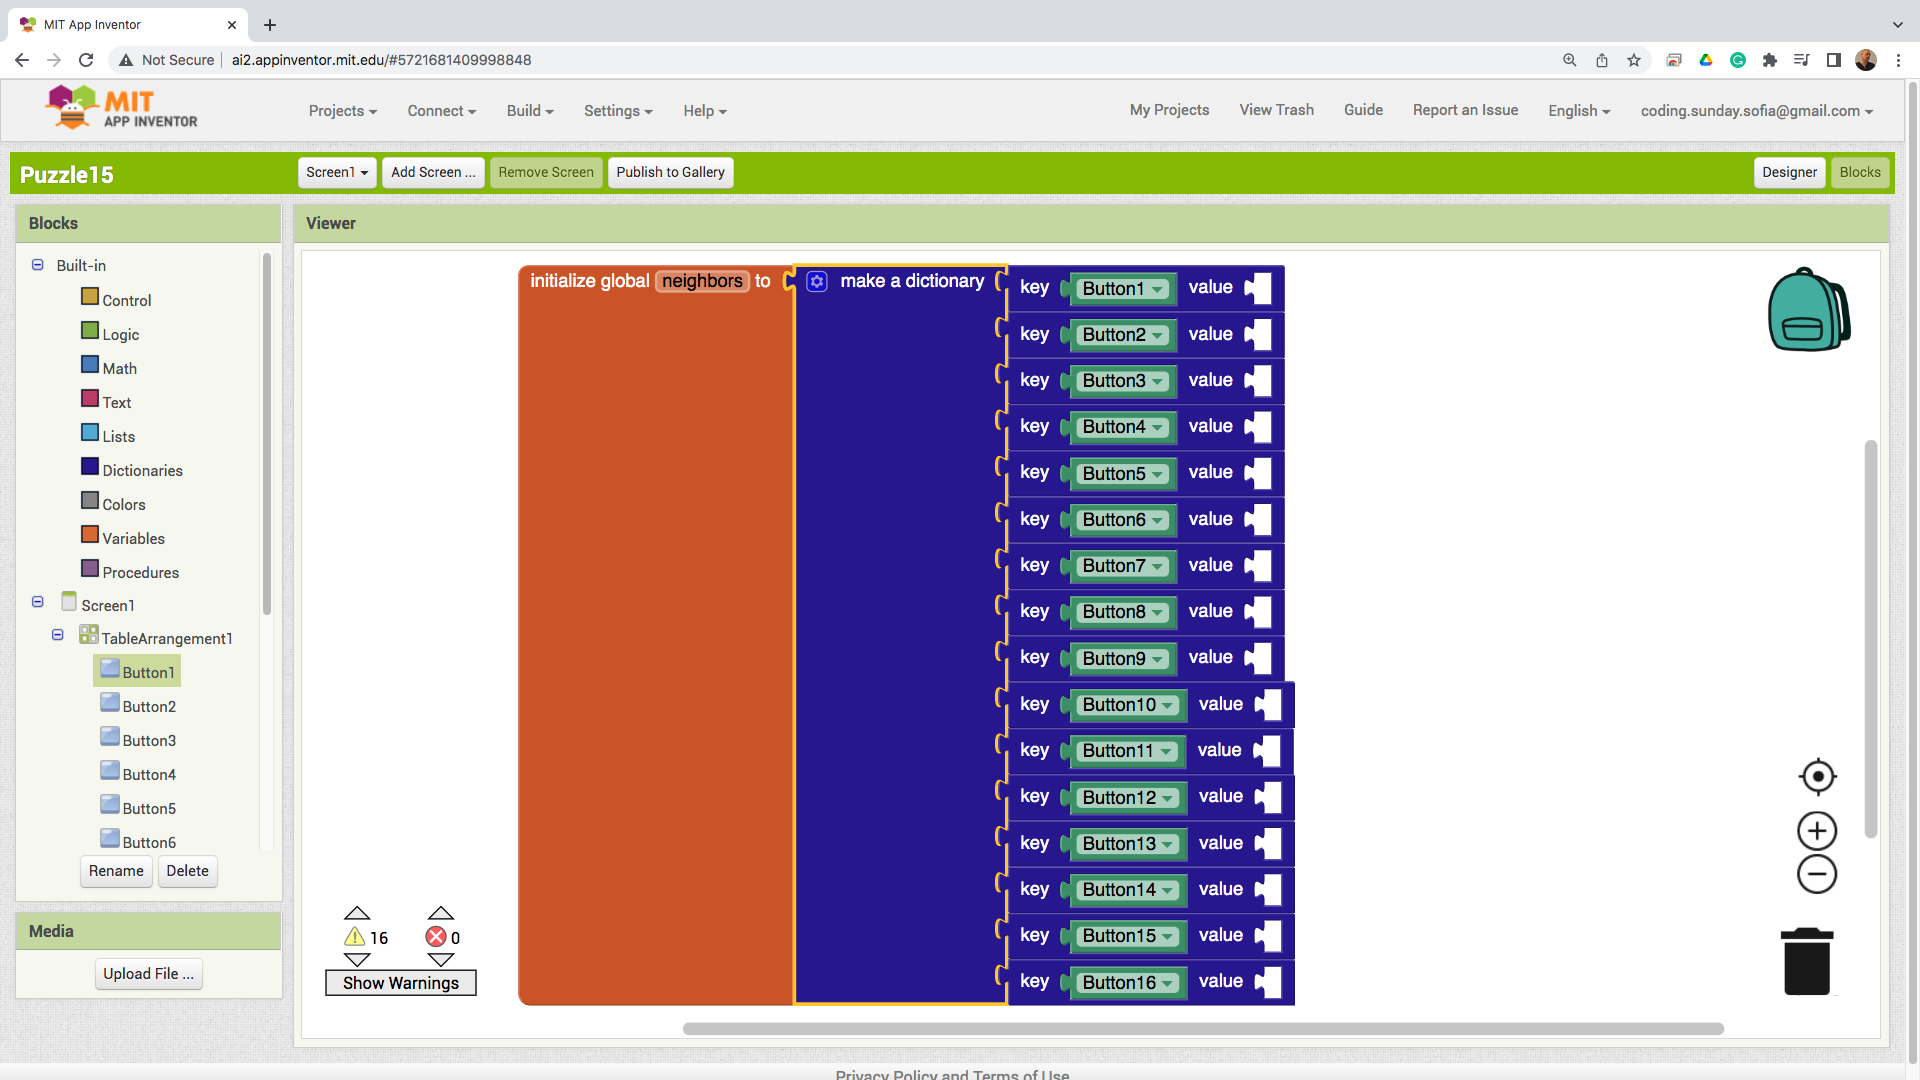
\includegraphics[width=1.0\linewidth,height=0.5\linewidth]{fig060005.png}
  \caption{Бутоните като ключови стойности}
\label{fig060005}
\end{figure}

Този речник на съответствията става достъпен като глобална променлива, така че да се ползва в различните събития от визуалния интерфейс. Бутон едно за съседи има бутон две и бутон пет  (Фиг. \ref{fig060006}). 

\begin{figure}[H]
  \centering
  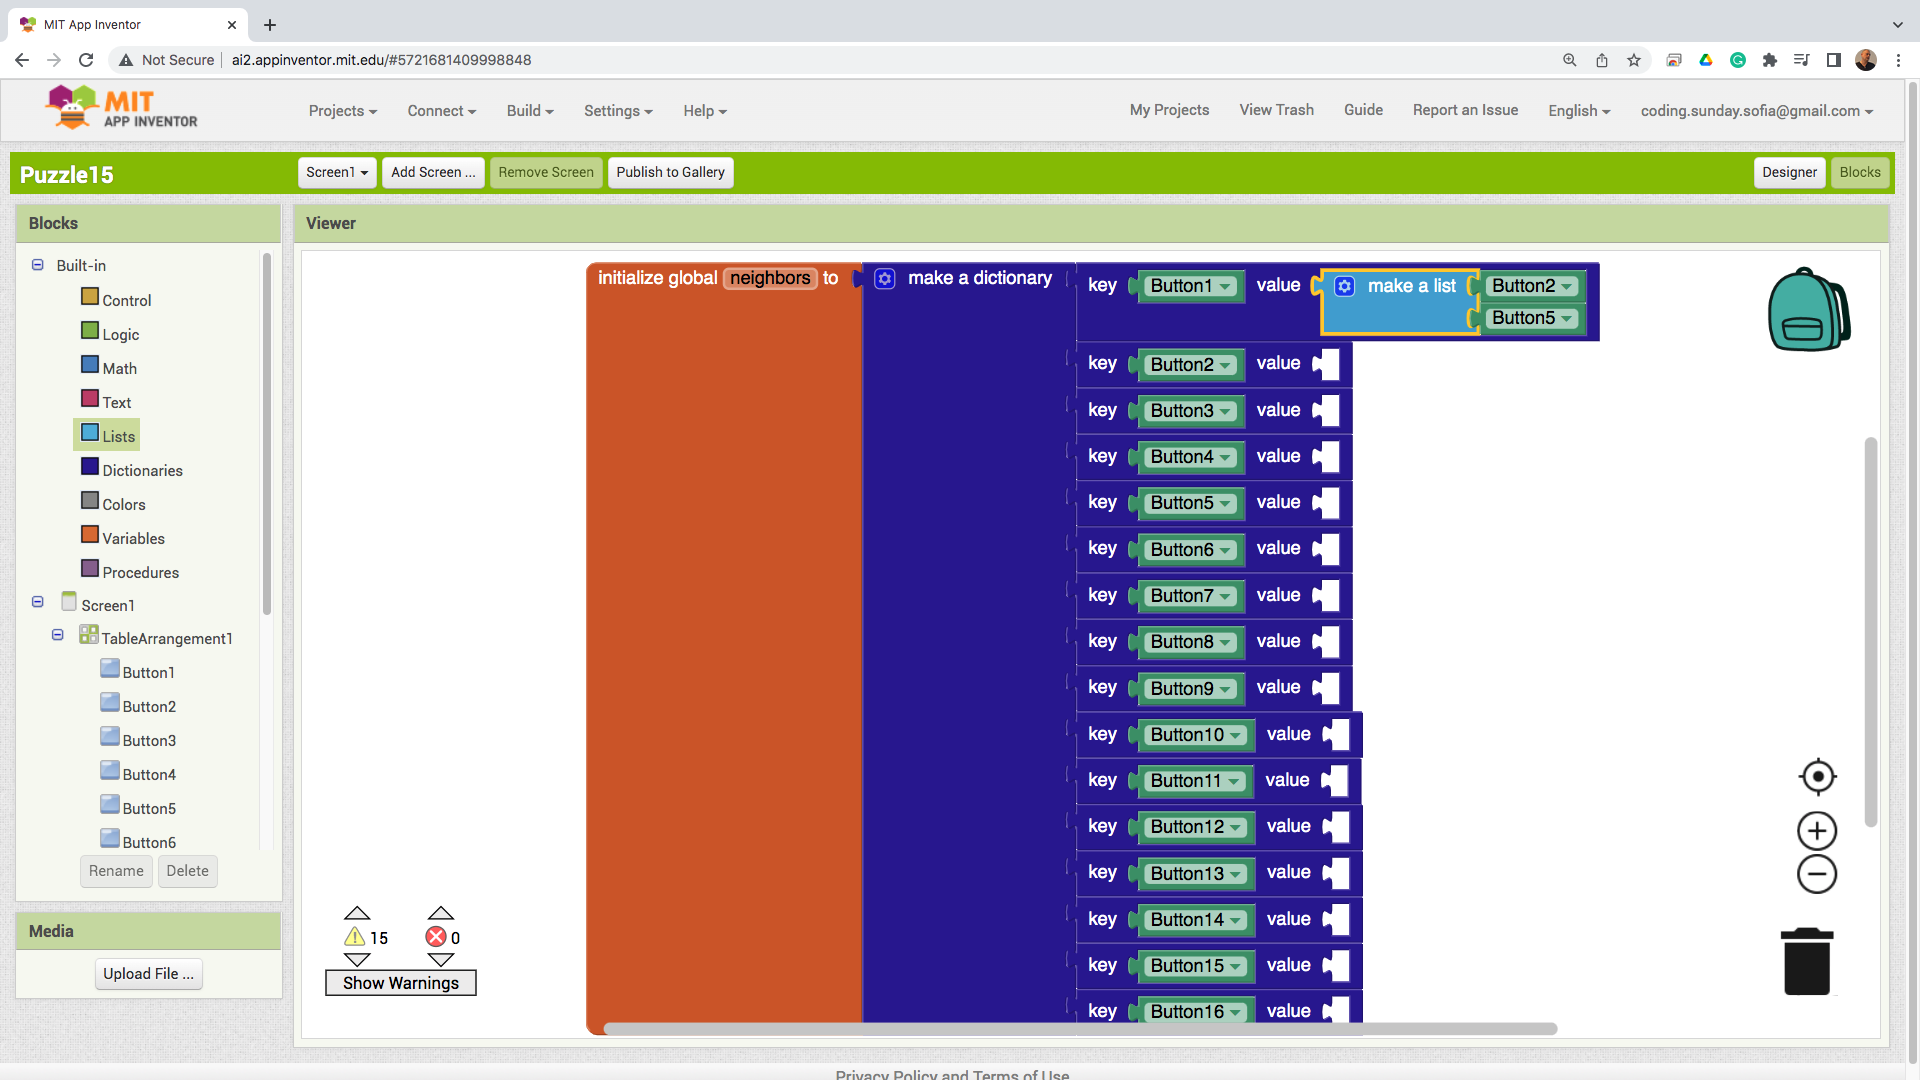
\includegraphics[width=1.0\linewidth,height=0.5\linewidth]{fig060006.png}
  \caption{Бутони като списък от съседи}
\label{fig060006}
\end{figure}

Бутон две има за съседи бутон едно, шест и три. Съседи на бутон три са две, седем и четири. Съседи на бутон четири са три и осем. Съседи на бутон пет са едно, шест и девет. Съседи на бутон шест са две, пет, седем и десет. Съседи на бутон седем са три, шест, осем и единадесет. Съседи на бутон осем са четири, седем и дванадесет. Съседи на бутон девет са пет, десет и тринадесет. Съседи на бутон десет са шест, девет, единадесет и четиринадесет. Съседи на бутон единадесет са седем, десет, дванадесет и петнадесет. Съседи на бутон дванадесет са осем, единадесет и шестнадесет. Съседи на бутон тринадесет са девет и четиринадесет. Съседи на бутон четиринадесет са десет, тринадесет и петнадесет. Съседи на бутон петнадесет са единадесет, четиринадесет и шестнадесет. Съседи на бутон шестнадесет са дванадесет и петнадесет. Списъците за съседство се попълват по идентичен начин (Фиг. \ref{fig060007}).

\begin{figure}[H]
  \centering
  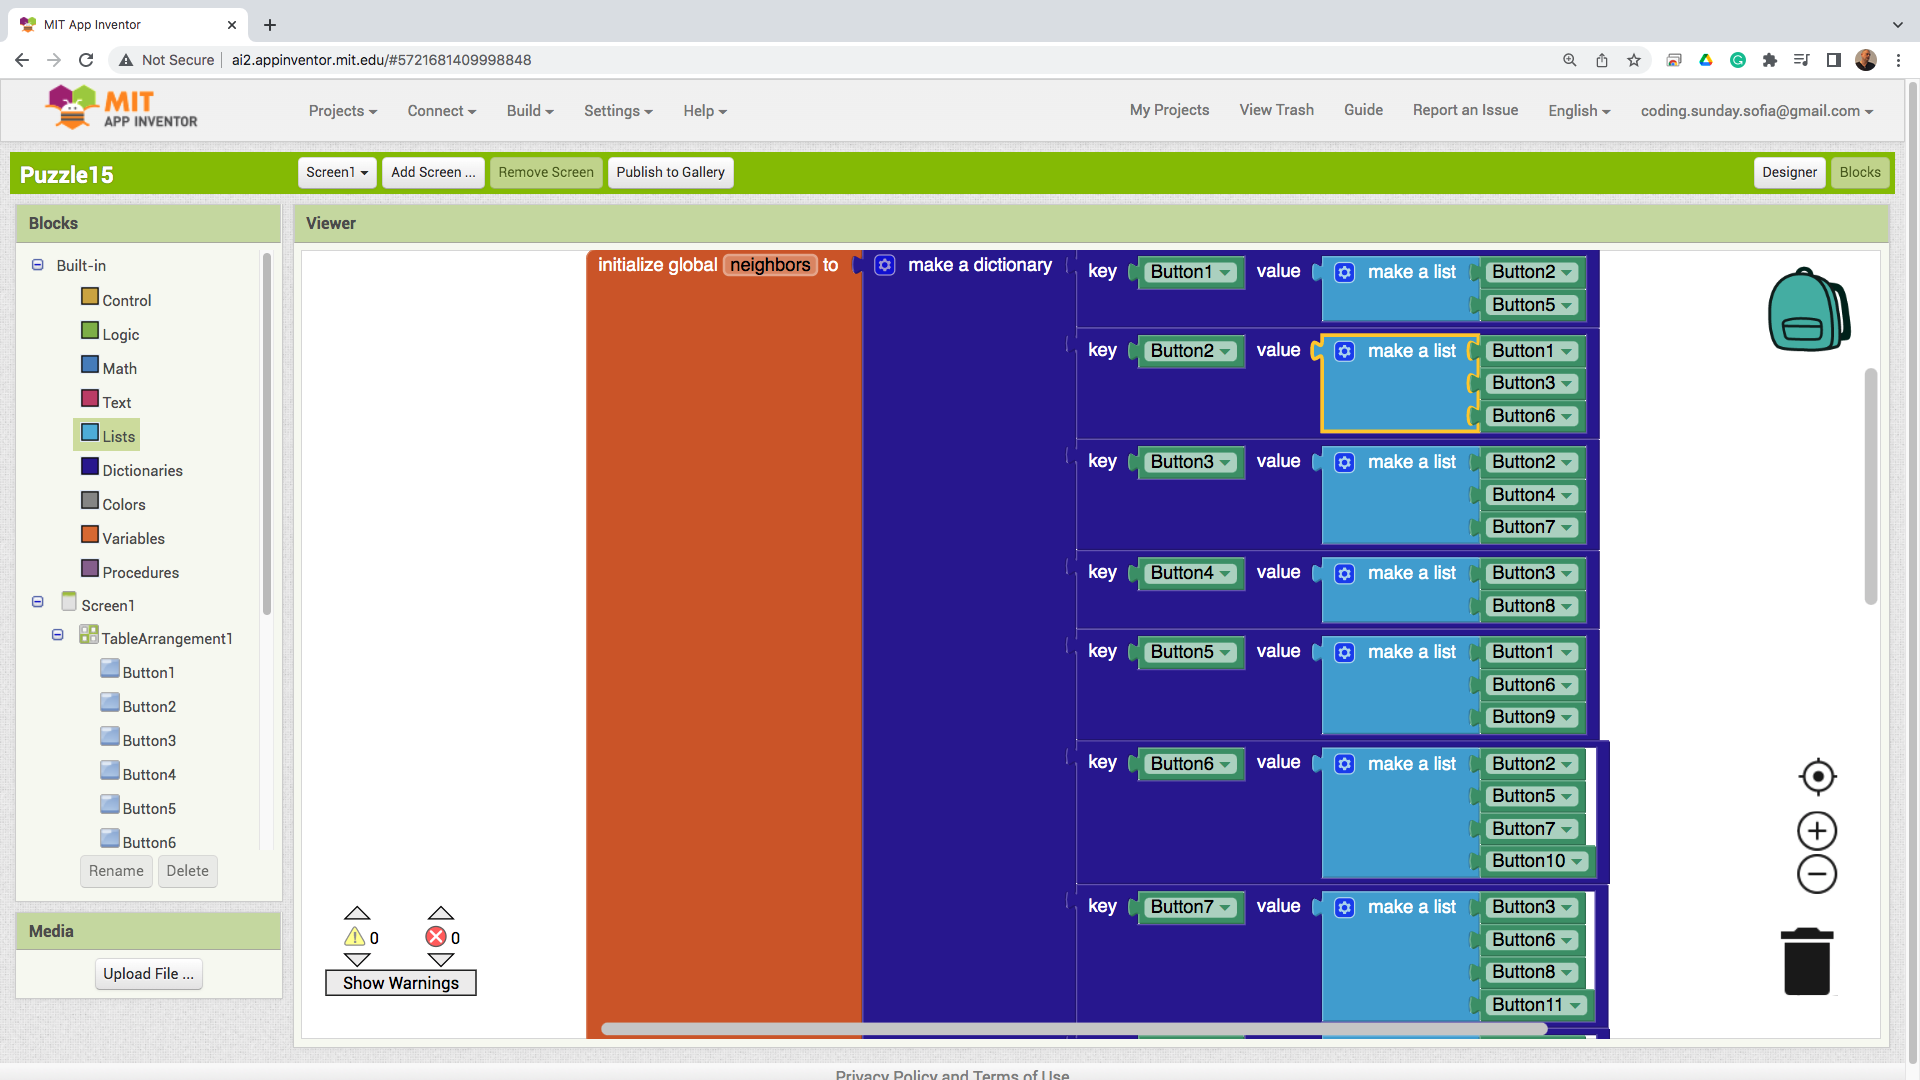
\includegraphics[width=1.0\linewidth,height=0.5\linewidth]{fig060007.png}
  \caption{Идентично попълване на съседните бутони}
\label{fig060007}
\end{figure}

Натискането на който и да е от бутоните предизвика събитие, което е общо за всички бутони (Фиг. \ref{fig060008}). Тъй като не е определено кой бутон ще натисне потребителя, то се прави проверка за натиснатия бутон (идва като параметър на събитието). 

\begin{figure}[H]
  \centering
  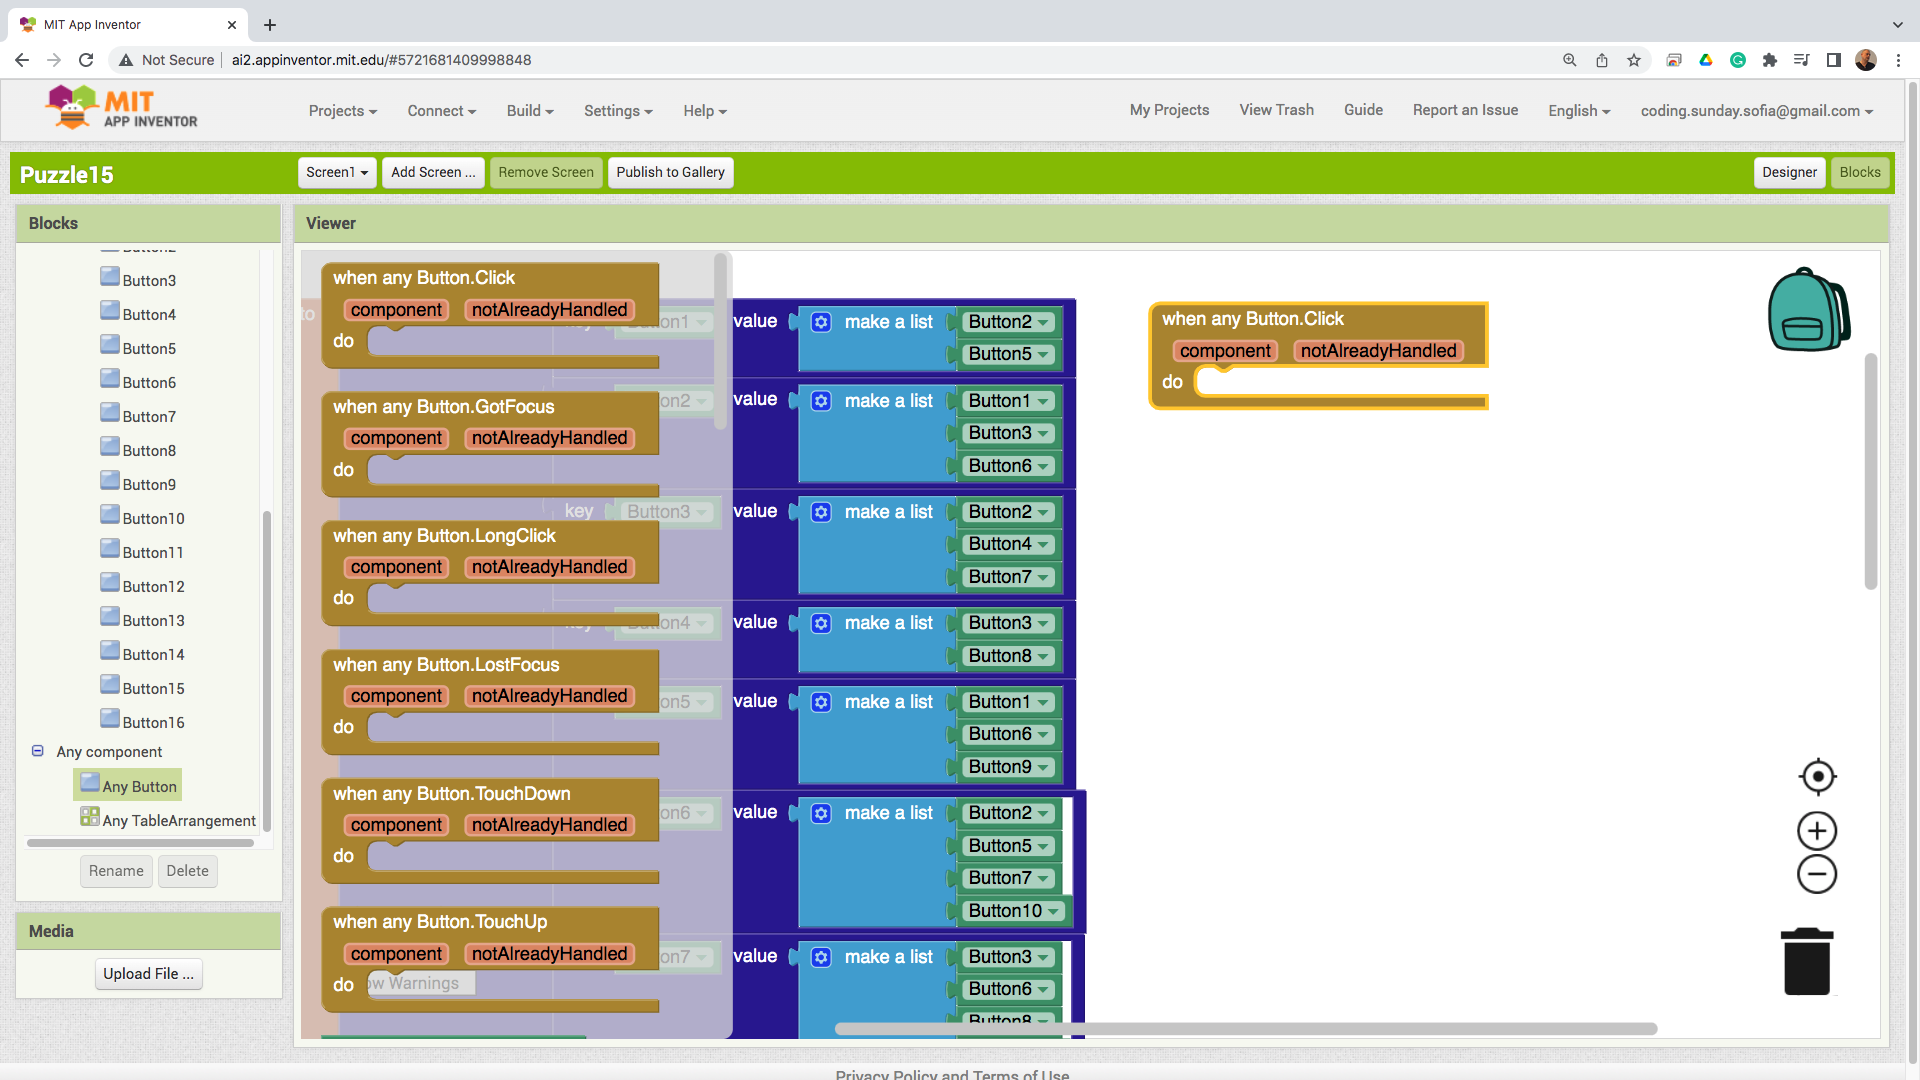
\includegraphics[width=1.0\linewidth,height=0.5\linewidth]{fig060008.png}
  \caption{Събитие за натиснат бутон}
\label{fig060008}
\end{figure}

Проверката дали празната клетка е съседство и евентуалната размяна с празната клетка се поверява на допълнителна процедура (Фиг. \ref{fig060009}). Процедурата получава като входен параметър компонента, предизвикал събитието. 

\begin{figure}[H]
  \centering
  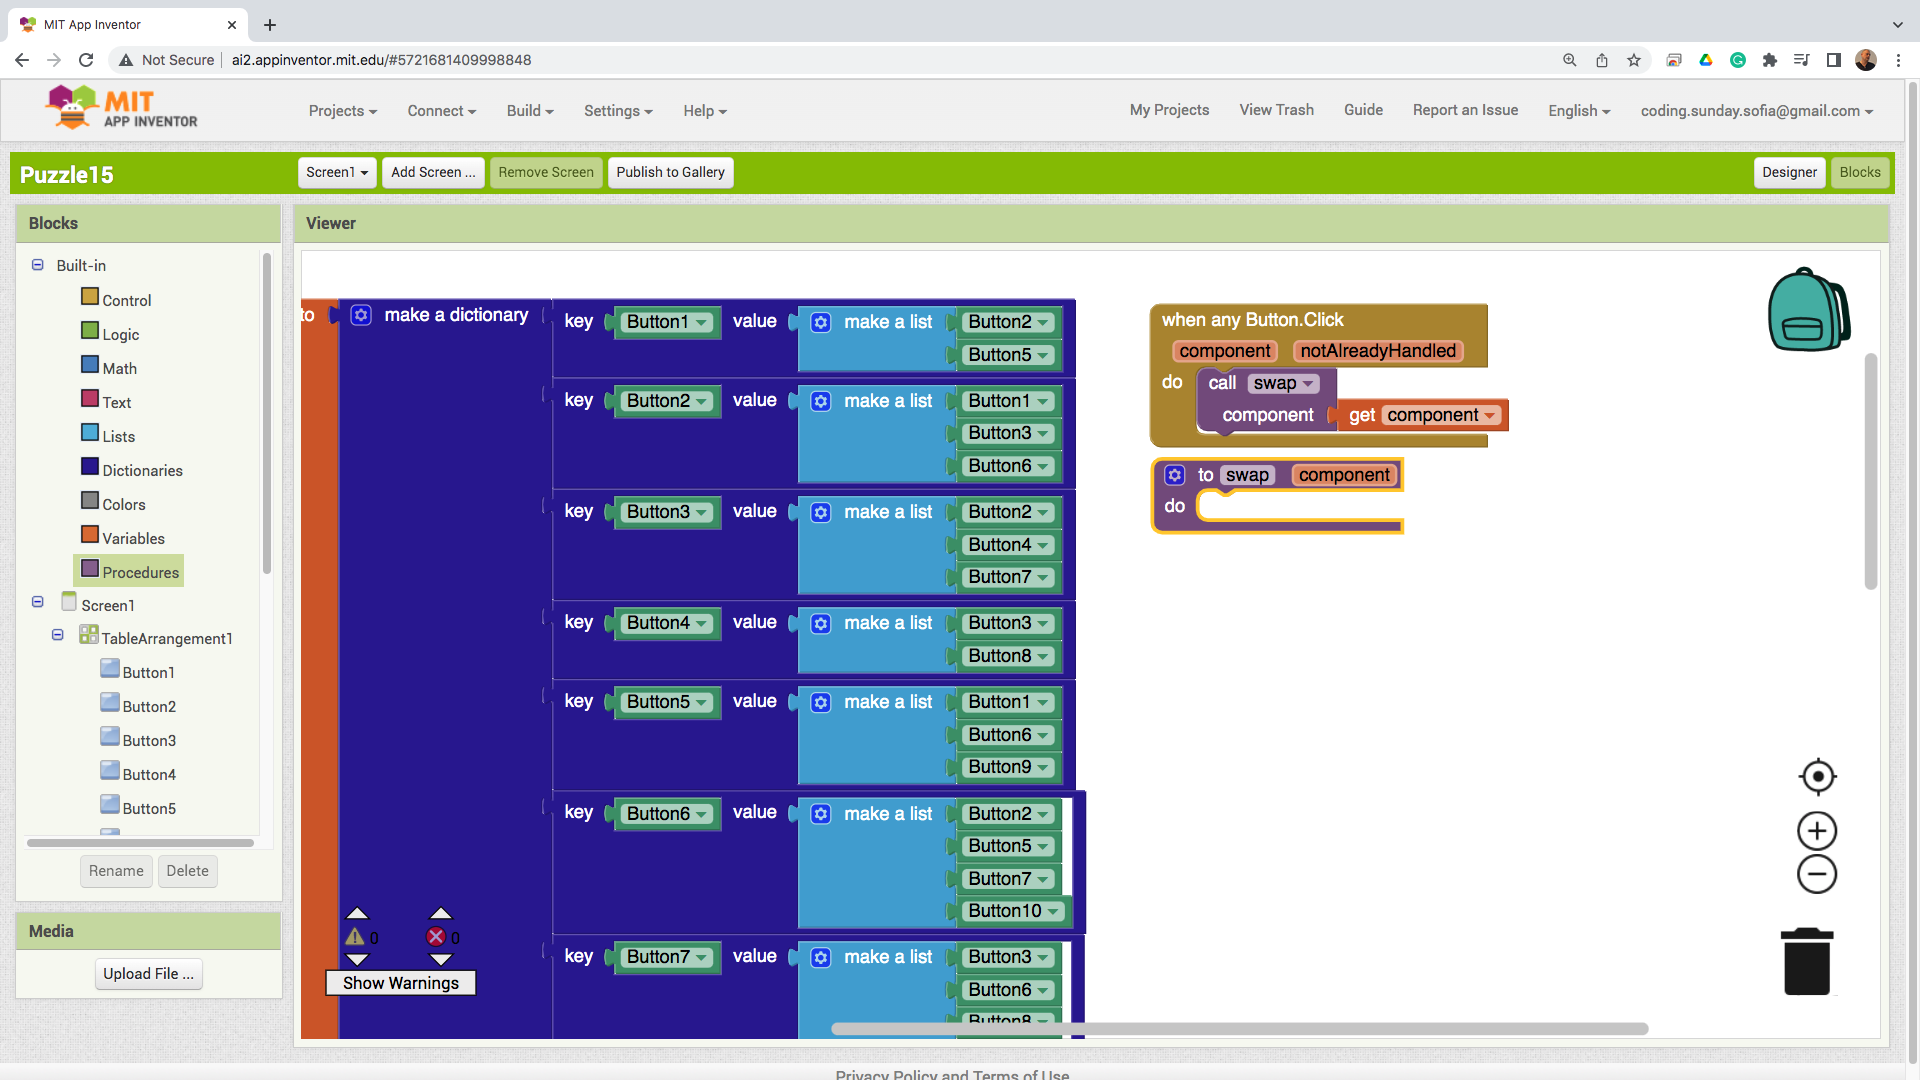
\includegraphics[width=1.0\linewidth,height=0.5\linewidth]{fig060009.png}
  \caption{Процедура за размяна}
\label{fig060009}
\end{figure}

За да се определи дали празната клетка е в съседство на натиснатия бутон се проверява целият списък, който се намира в речника на ключова позиция, посочена от компонента предизвикал събитието. Тази проверка е възможна с цикъл за обхождане на елементите в списъчна структура (Фиг. \ref{fig060010}). Ключовата стойност би трябвало винаги да връща списък със съседните бутони, но ако ключът не е намерен, за безопасност, се връща празен списък.

\begin{figure}[H]
  \centering
  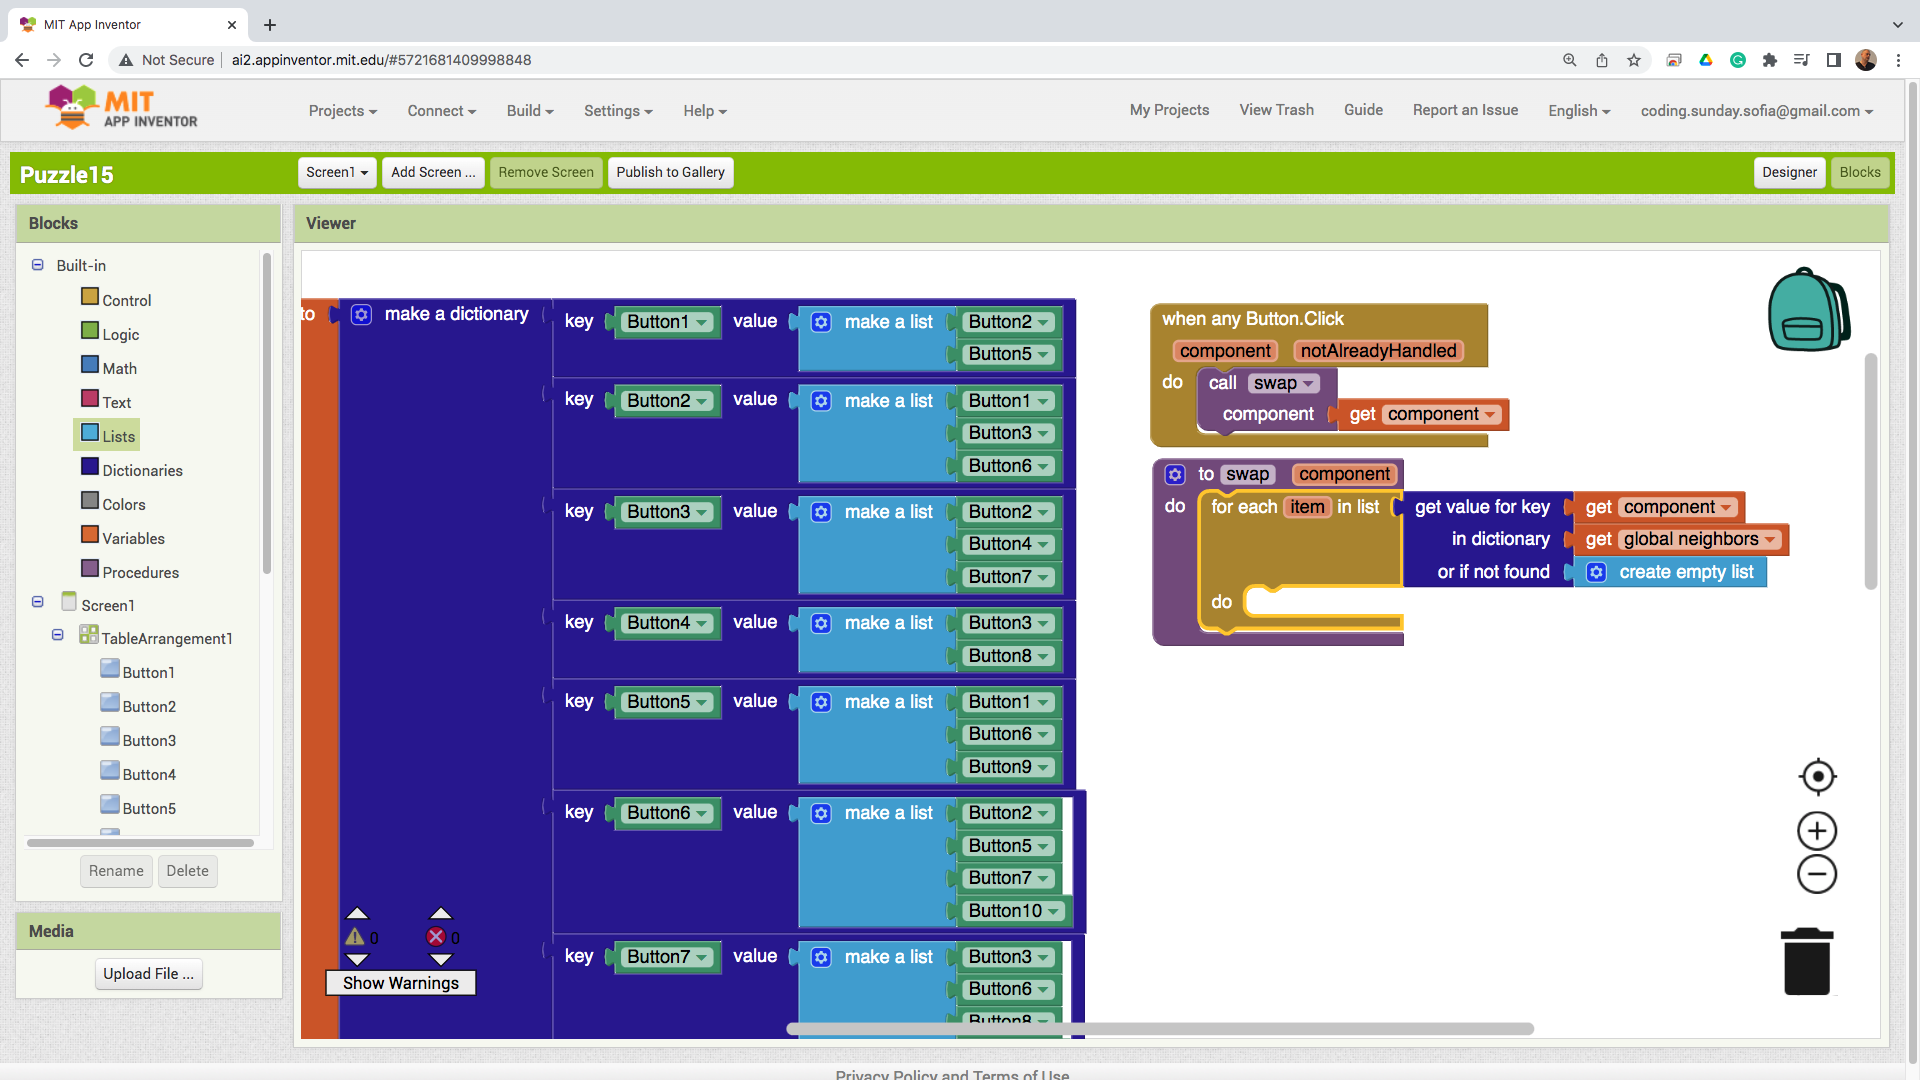
\includegraphics[width=1.0\linewidth,height=0.5\linewidth]{fig060010.png}
  \caption{Цикъл за обхождане на съседите}
\label{fig060010}
\end{figure}

Размяна с прави само, ако в списъка бъде открита празната клетка. Направата на размяната спира и цикъла за търсене на празната клетка. Условието съседен бутон да обозначава праната клетка е неговият надпис да бъде два интервала (Фиг. \ref{fig060011}). 

\begin{figure}[H]
  \centering
  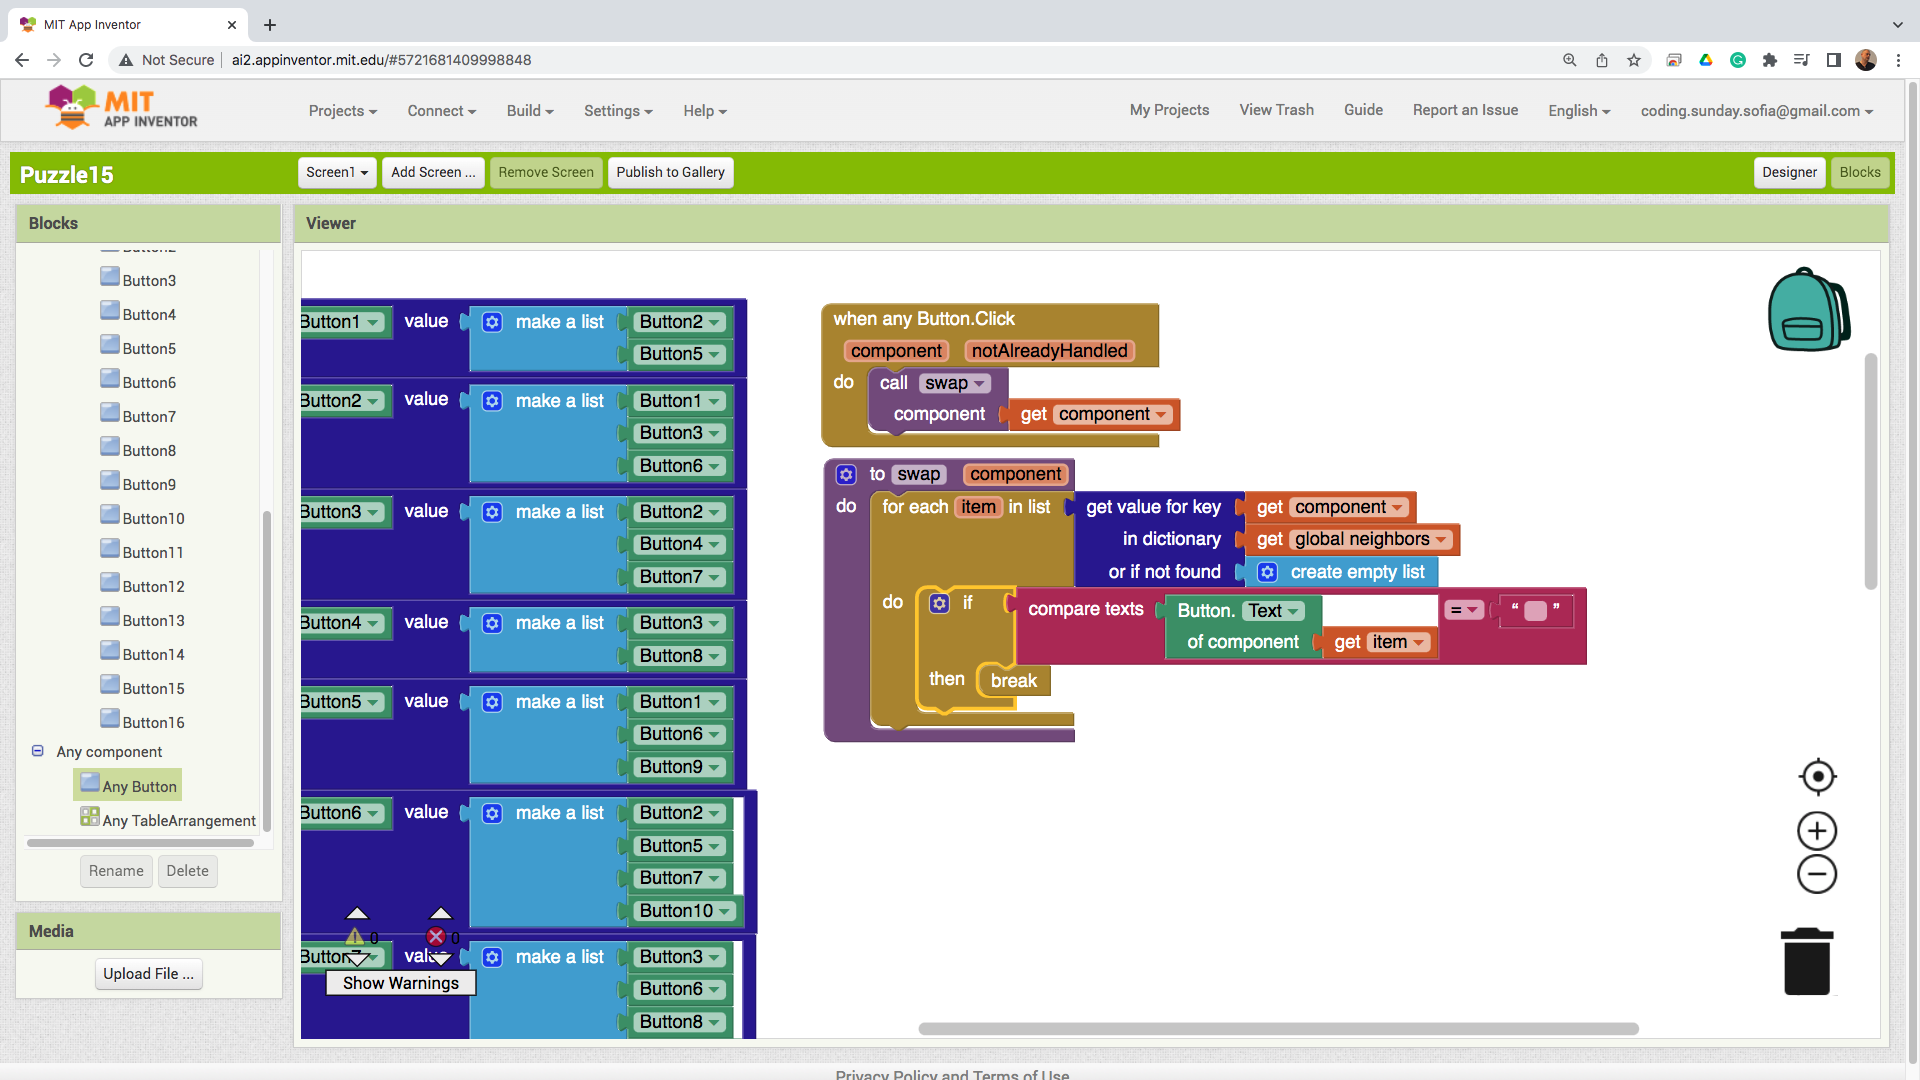
\includegraphics[width=1.0\linewidth,height=0.5\linewidth]{fig060011.png}
  \caption{Проверка за празната клетка}
\label{fig060011}
\end{figure}

За улесняване на размяната се залагат четири локални, помощни променливи. Две променливи за текстовете на двата бутона и две променливи за цветовете на текстовете (Фиг. \ref{fig060012}).

\begin{figure}[H]
  \centering
  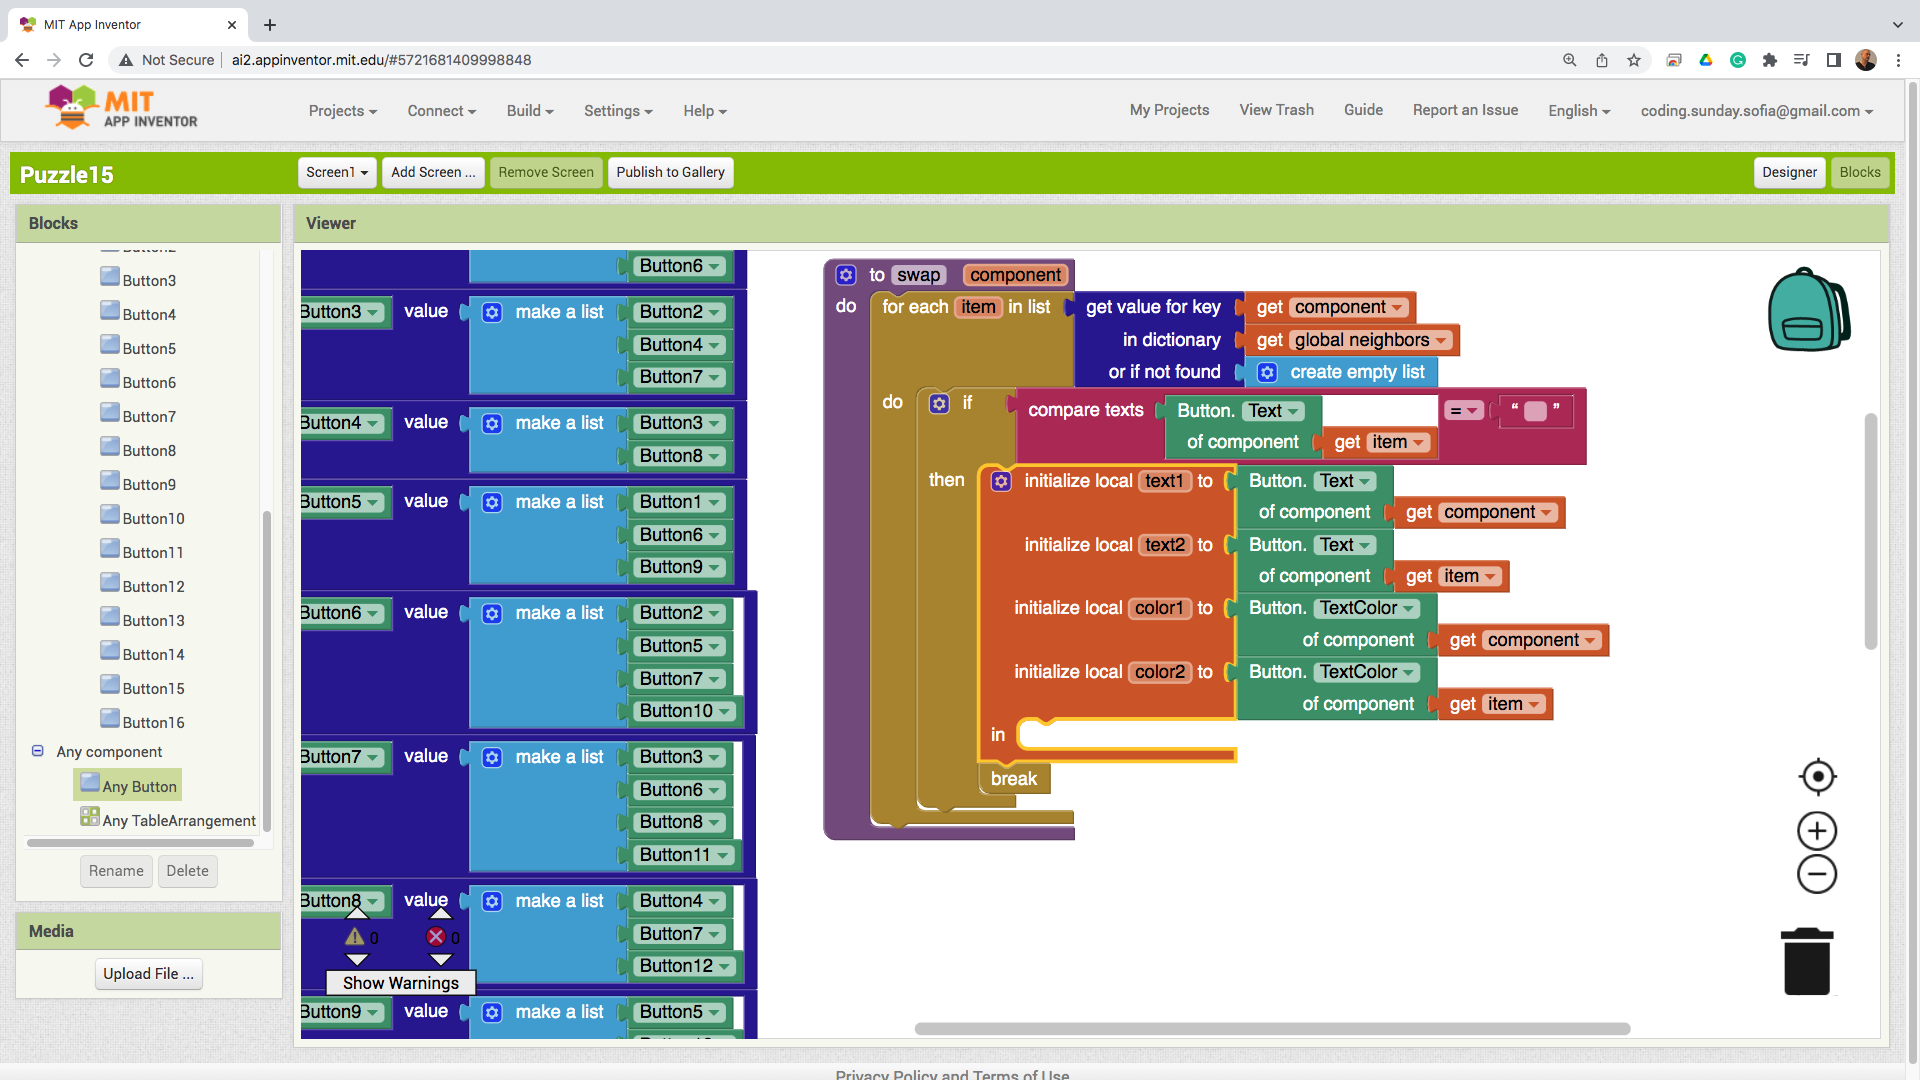
\includegraphics[width=1.0\linewidth,height=0.5\linewidth]{fig060012.png}
  \caption{Локални помощни променливи}
\label{fig060012}
\end{figure}

Размяната се осъществява, чрез записване на помощните променливи, като нови стойности за двата бутона (Фиг. \ref{fig060013}).

\begin{figure}[H]
  \centering
  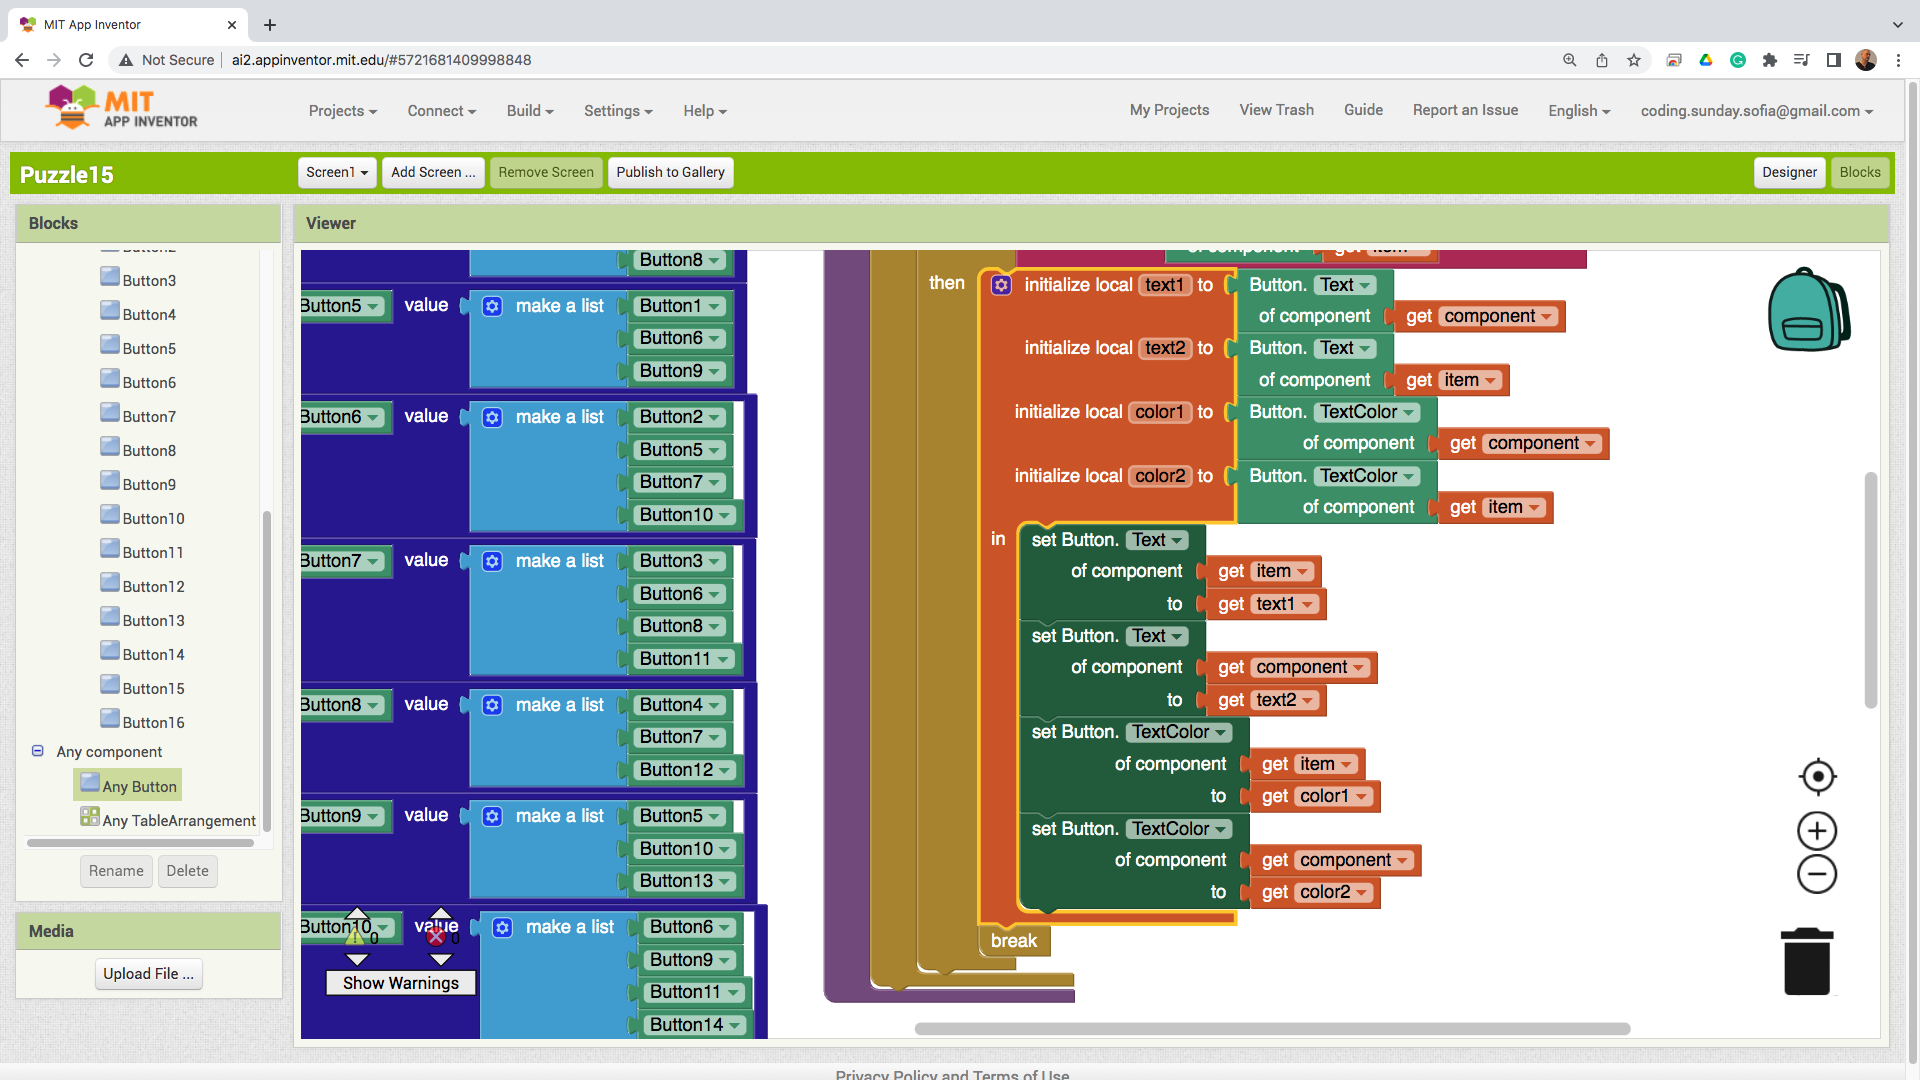
\includegraphics[width=1.0\linewidth,height=0.5\linewidth]{fig060013.png}
  \caption{Размяна на стойностите}
\label{fig060013}
\end{figure}

На този етап играта притежава абсолютно цялата функционалност, която притежава и механичната играчка (Фиг. \ref{fig060014}).

\begin{figure}[H]
  \centering
  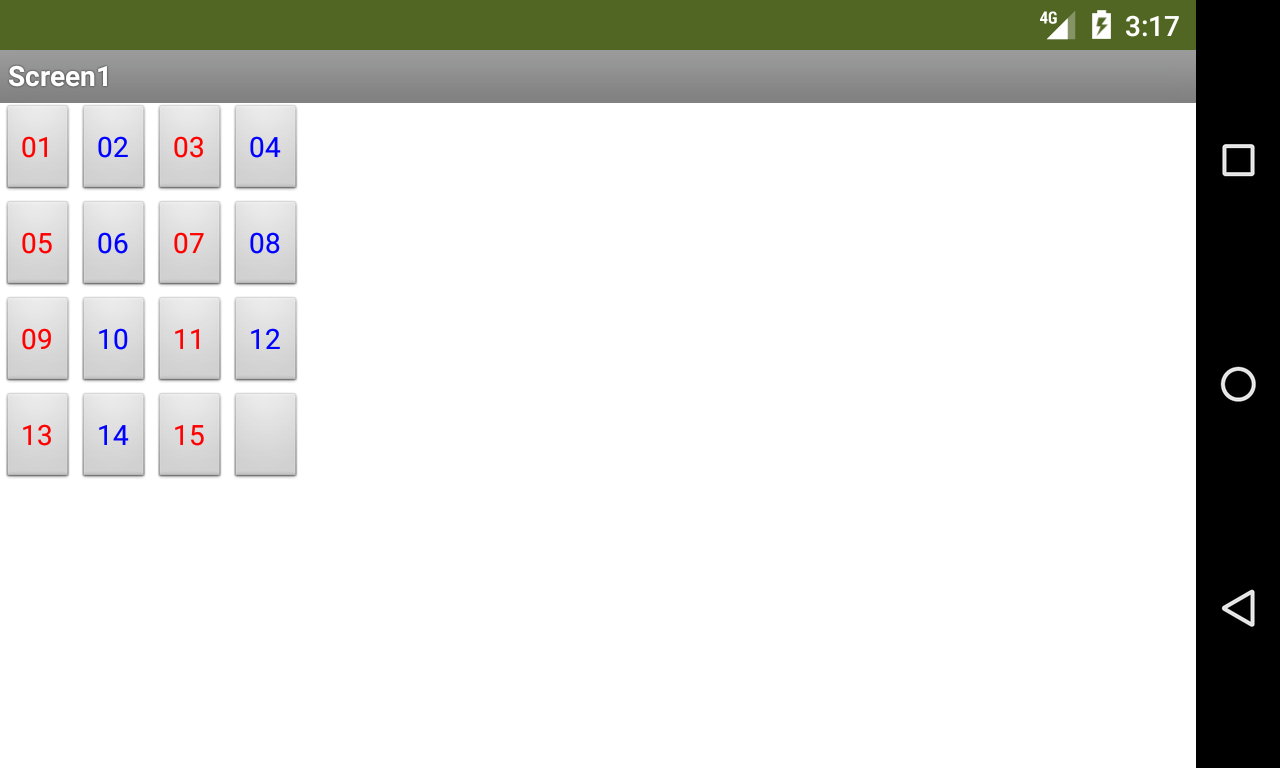
\includegraphics[width=1.0\linewidth,height=0.5\linewidth]{fig060014.png}
  \caption{Завършен вид на играта}
\label{fig060014}
\end{figure}

Въпреки, че всичко необходимо е налично, използването на компютър позволява да се добави още една полезна функция, а именно – автоматично разбъркване на пъзела. Операционната система позволява да се прихване събитие за дълго натискане на бутон (Фиг. \ref{fig060015}).

\begin{figure}[H]
  \centering
  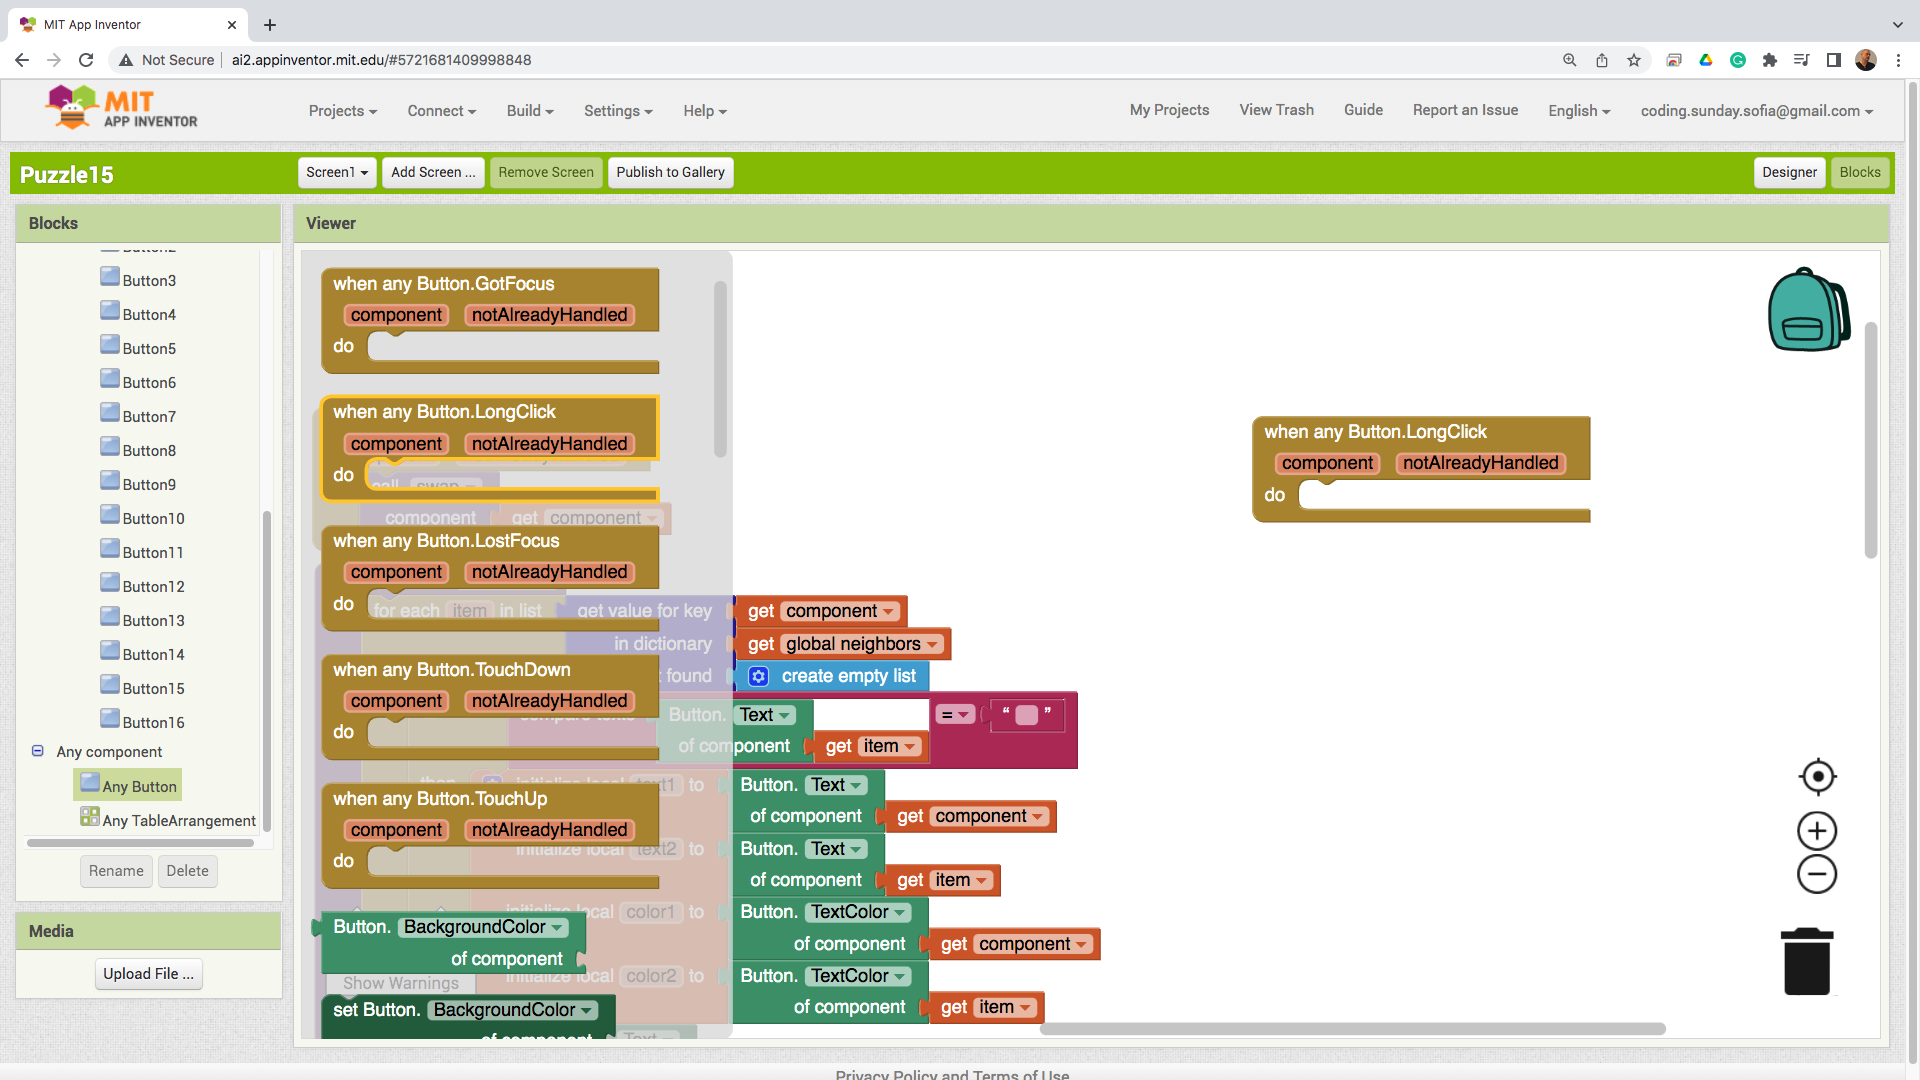
\includegraphics[width=1.0\linewidth,height=0.5\linewidth]{fig060015.png}
  \caption{Събитие за дълго натискане на бутон}
\label{fig060015}
\end{figure}

Бутонът за празната клетка не е натоварен с много действия и поради тази причина може да се използва точно като бутон за разбъркване, стига да бъде натиснат за продължително време (Фиг. \ref{fig060016}).

\begin{figure}[H]
  \centering
  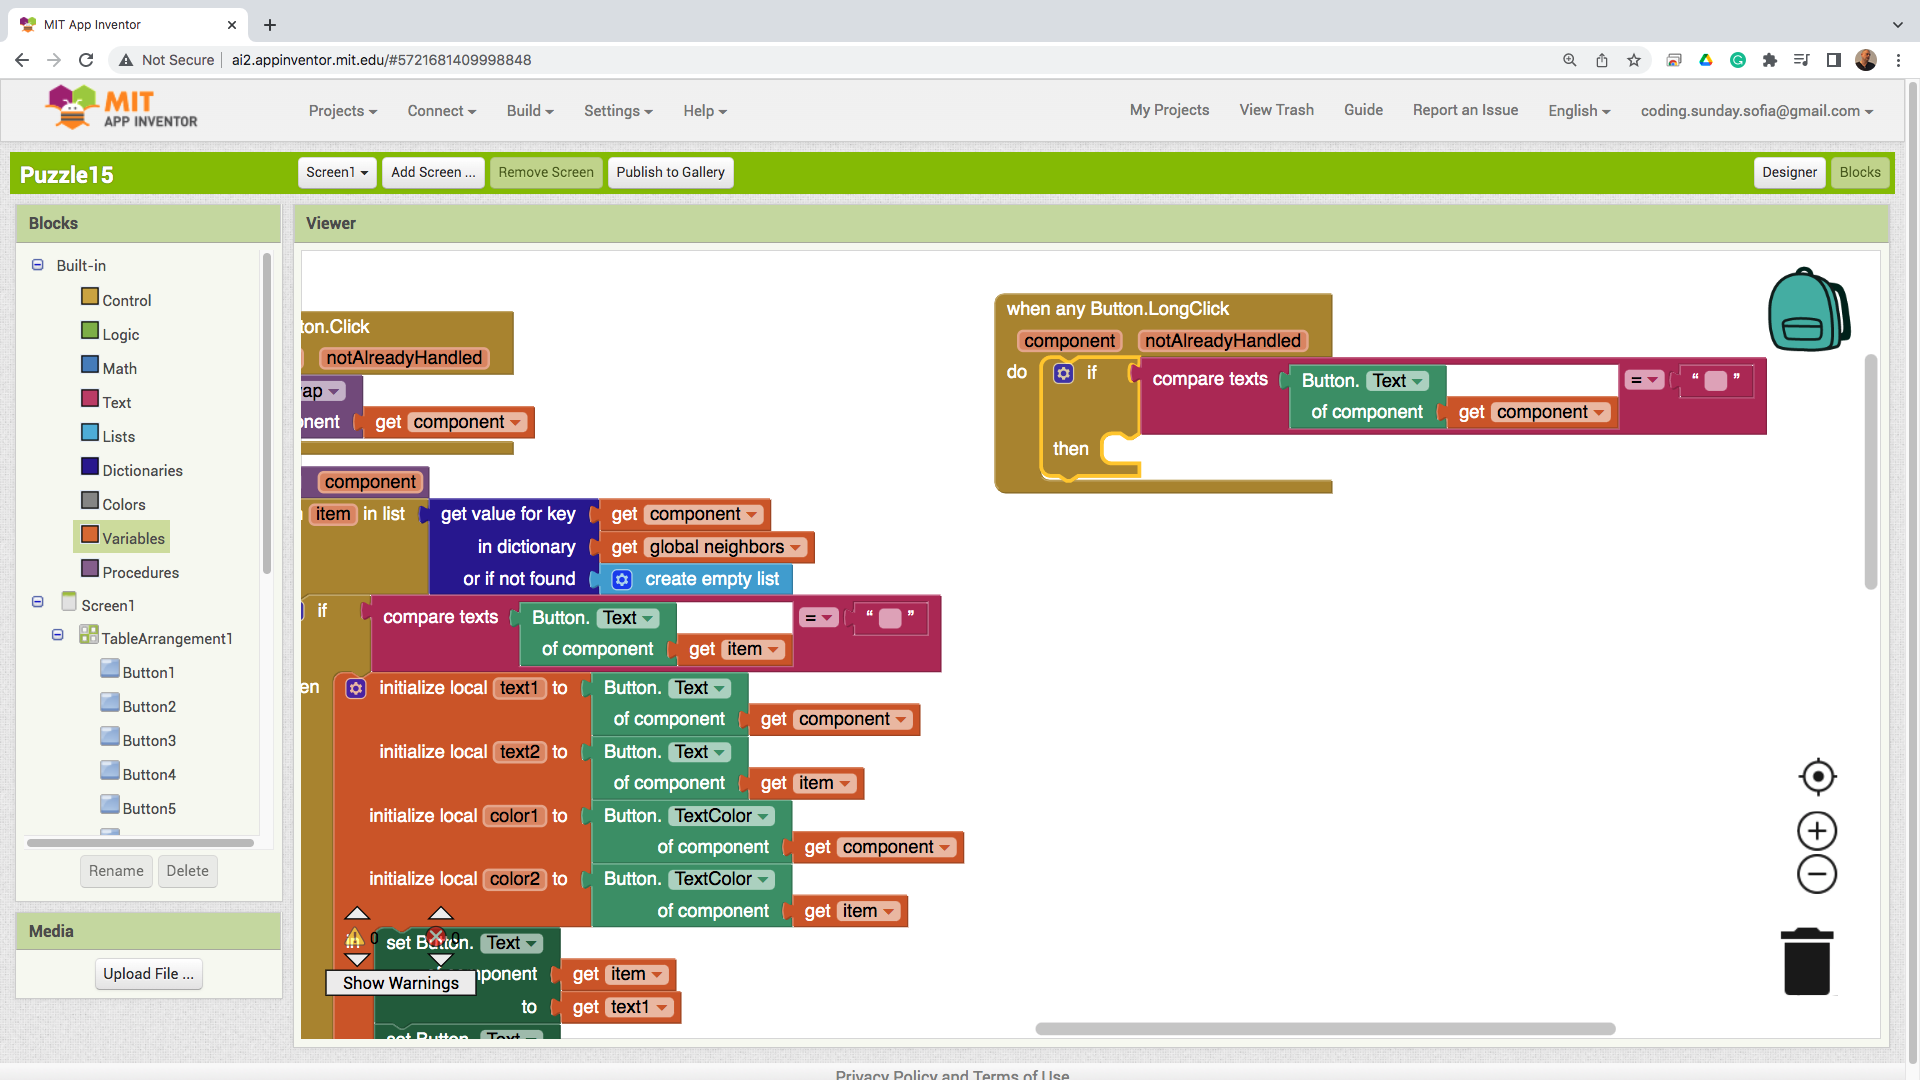
\includegraphics[width=1.0\linewidth,height=0.5\linewidth]{fig060016.png}
  \caption{Активиране на разбъркването}
\label{fig060016}
\end{figure}

Тъй като при разбъркването празната клетка ще се мести, то е добър вариант позицията й да се съхранява в локална, помощна променлива (Фиг. \ref{fig060017}).

\begin{figure}[H]
  \centering
  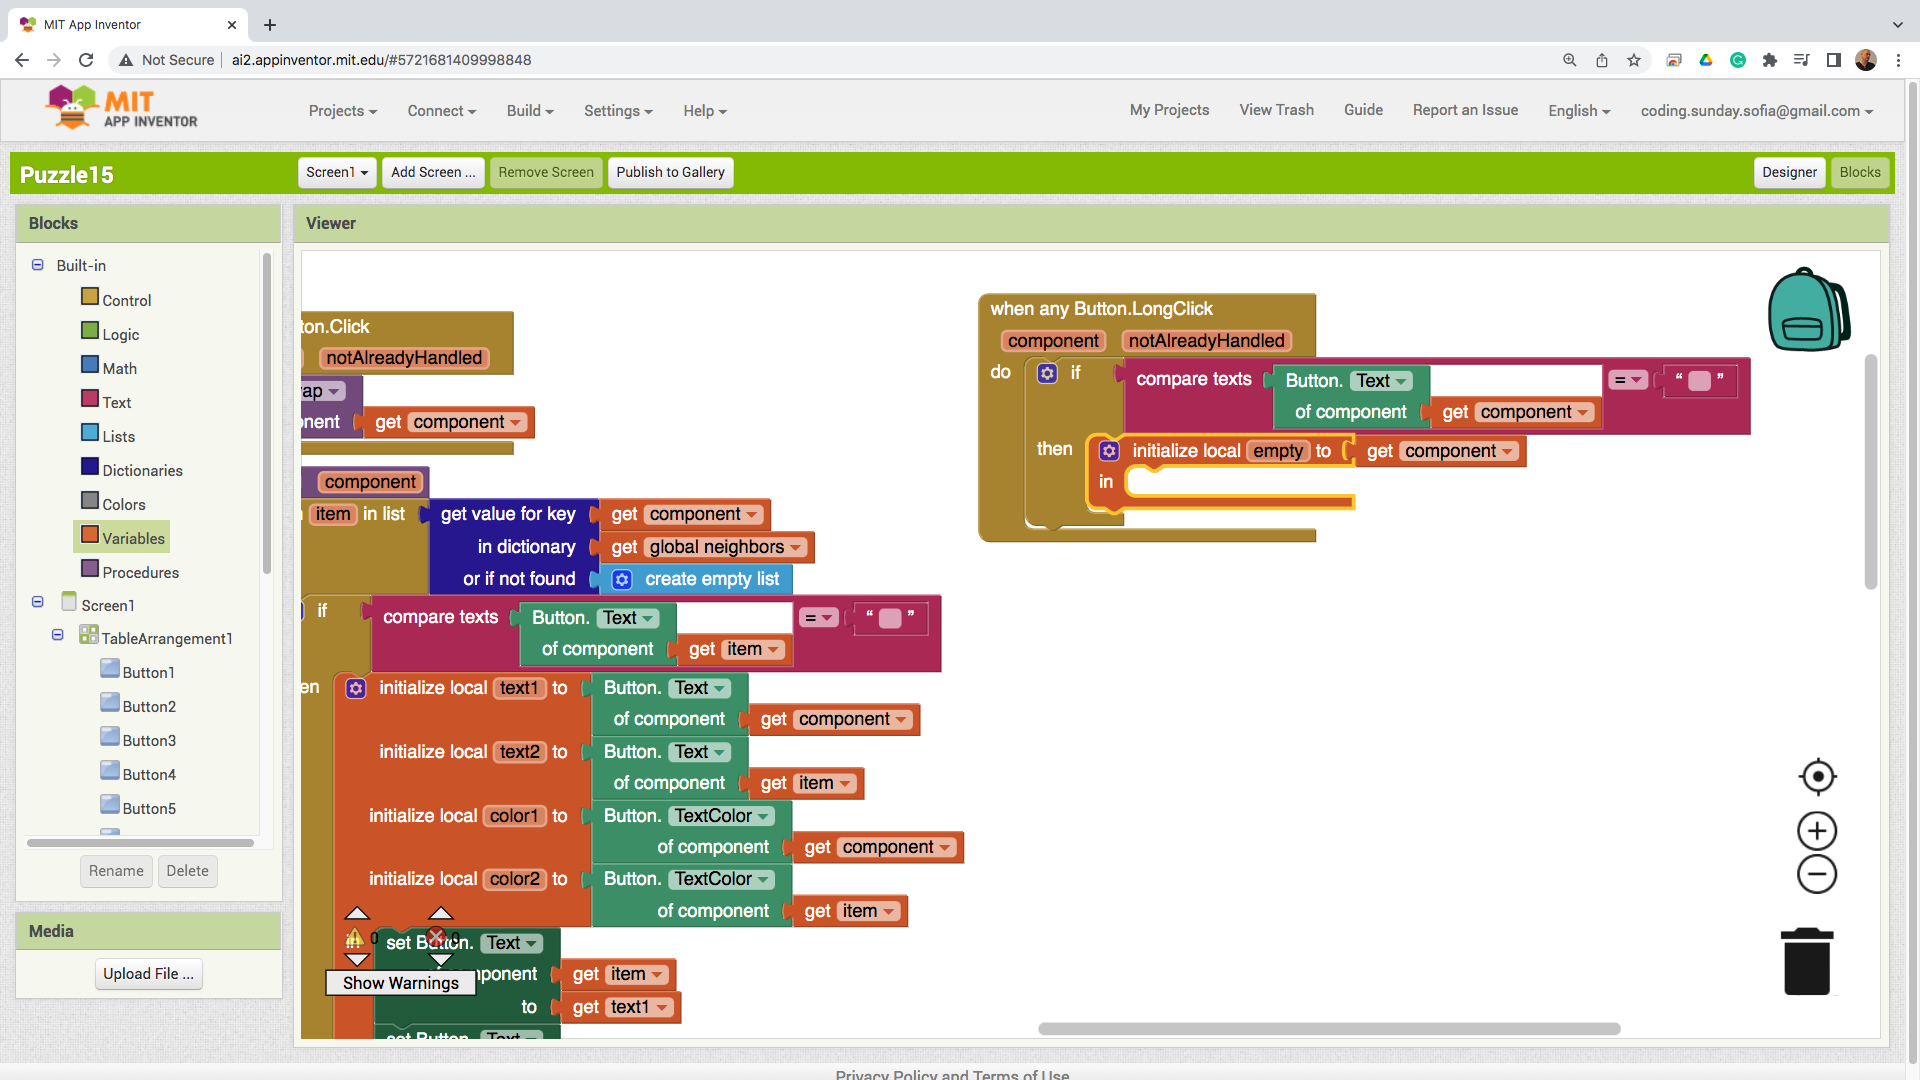
\includegraphics[width=1.0\linewidth,height=0.5\linewidth]{fig060017.png}
  \caption{Помощна променлива за позицията на празната клетка}
\label{fig060017}
\end{figure}

Игралното табло се състои от 16 позиции. За да може всяка позиция да участва, средно-статистически, 10 пъти в разбъркването, случайно избрани размествания могат да се направят 160 пъти, което е 16 клетки по десет пъти. За целта на разбъркването, цикъл с единична стъпка е най-удачната конструкция (Фиг. \ref{fig060018}).

\begin{figure}[H]
  \centering
  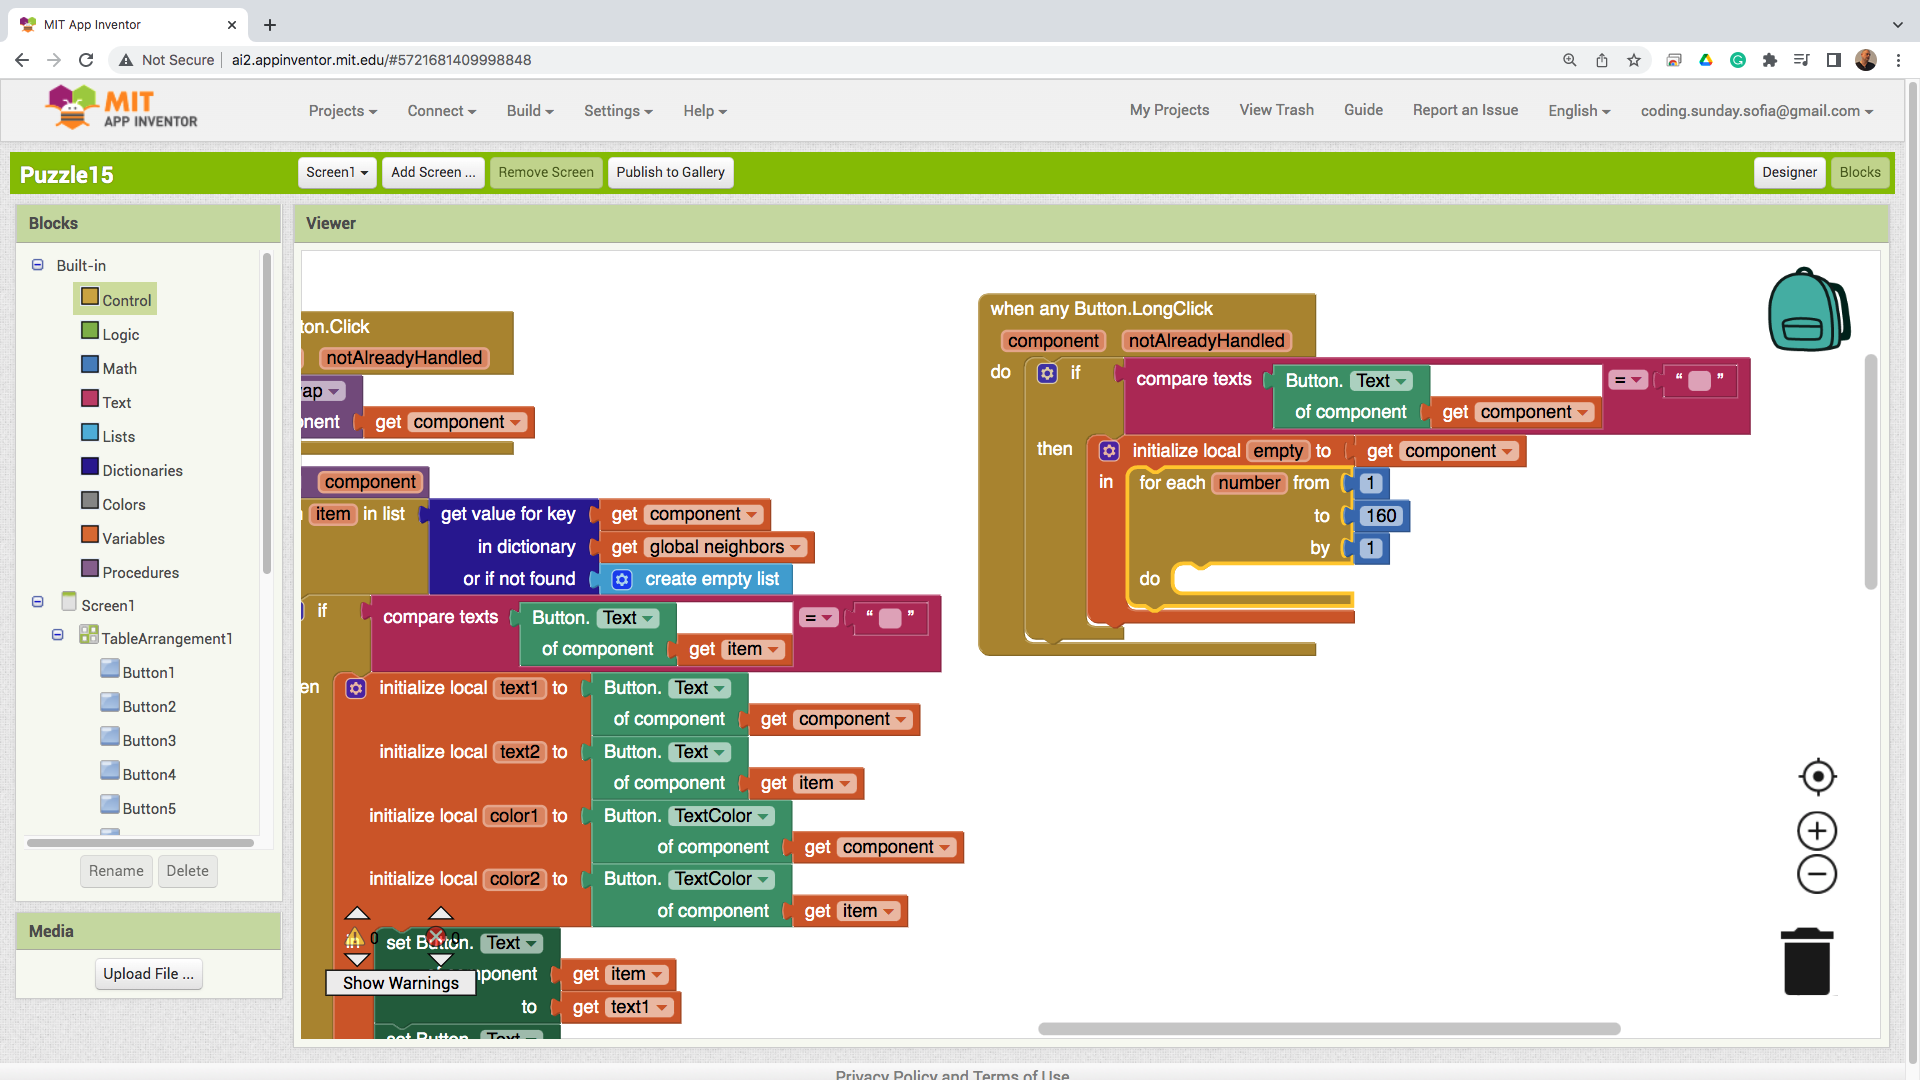
\includegraphics[width=1.0\linewidth,height=0.5\linewidth]{fig060018.png}
  \caption{Цикъл за разбъркване}
\label{fig060018}
\end{figure}

Изборът на следваща празна клетка се прави на случаен принцип от съседите на текущата празна клетка  (Фиг. \ref{fig060019}). Следващата празна клетка се записва във временна променлива, докато се извърши размяната.

\begin{figure}[H]
  \centering
  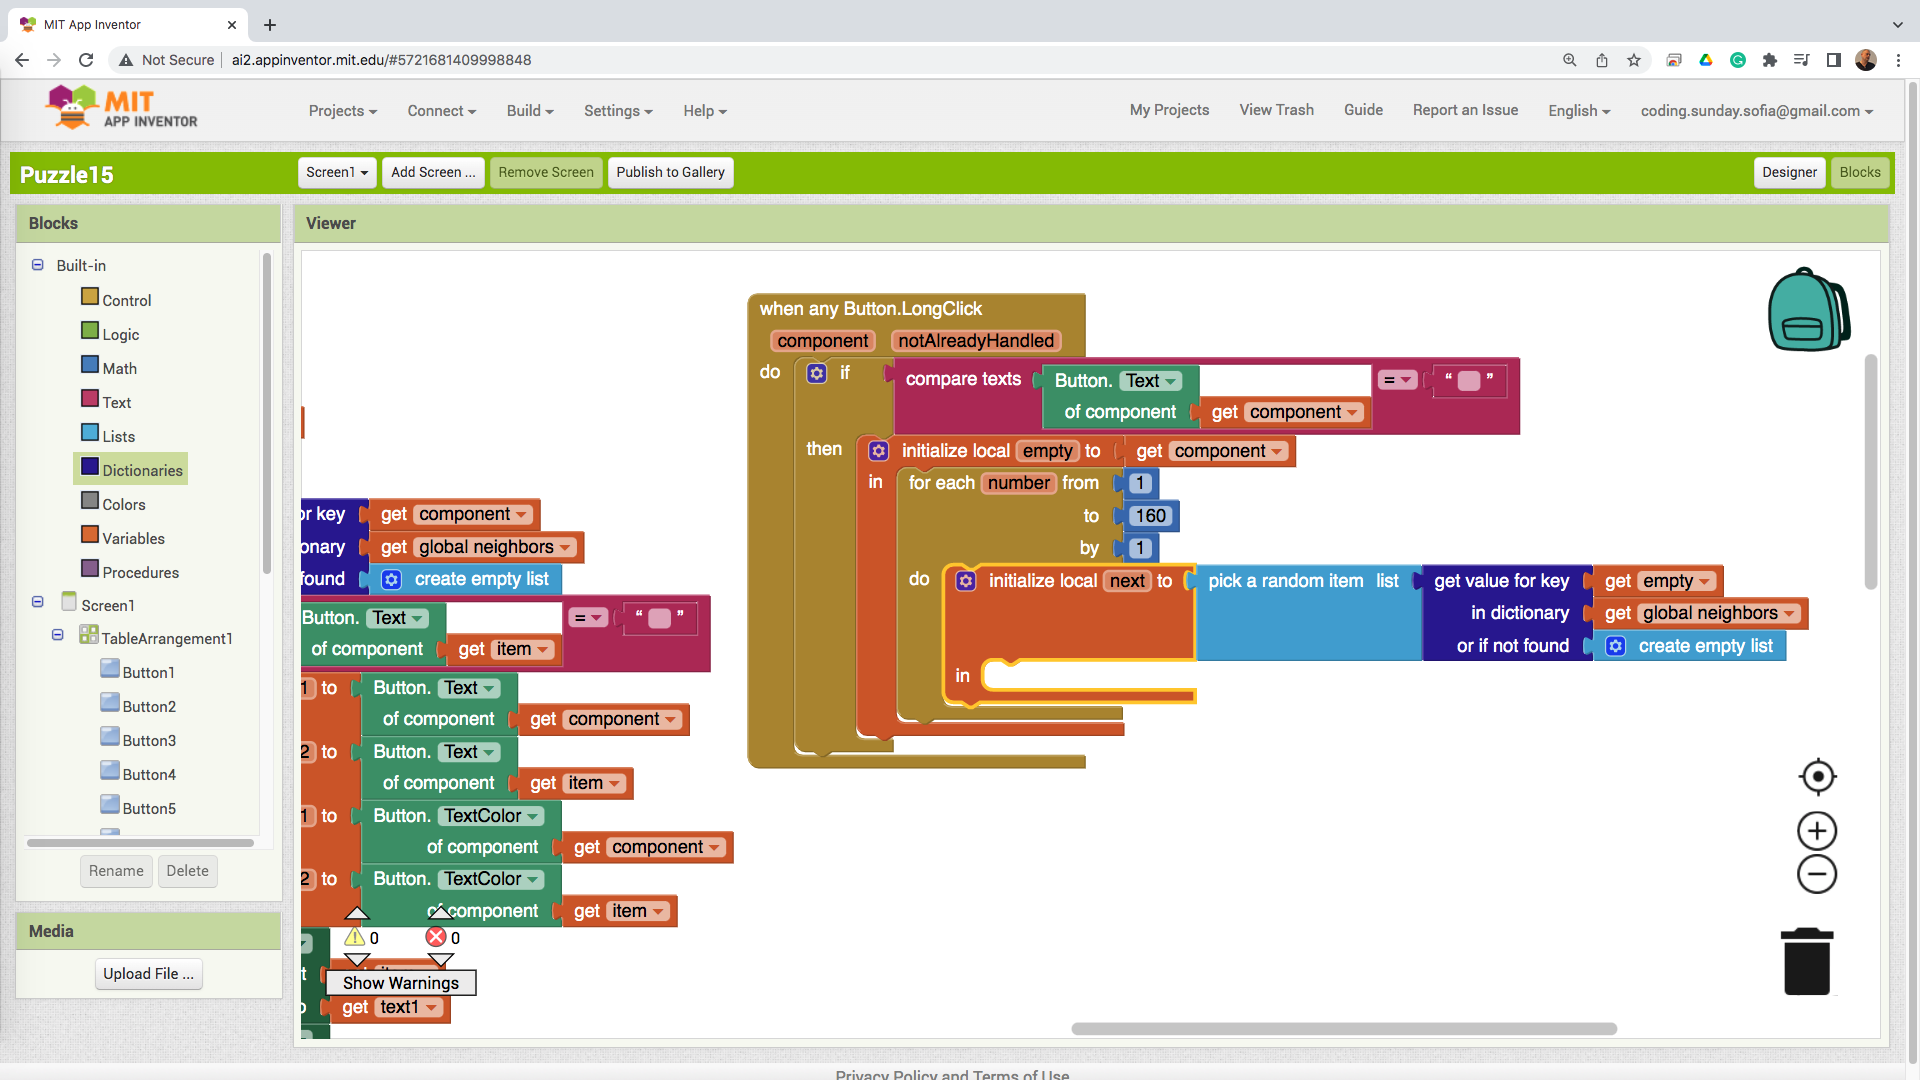
\includegraphics[width=1.0\linewidth,height=0.5\linewidth]{fig060019.png}
  \caption{Избор на случаен съсед на празната клетка}
\label{fig060019}
\end{figure}

Самата размяна се извършва с помощната процедура (Фиг. \ref{fig060020}). След размяната, празната клетка за следващото завъртане на цикъла се сменя.

\begin{figure}[H]
  \centering
  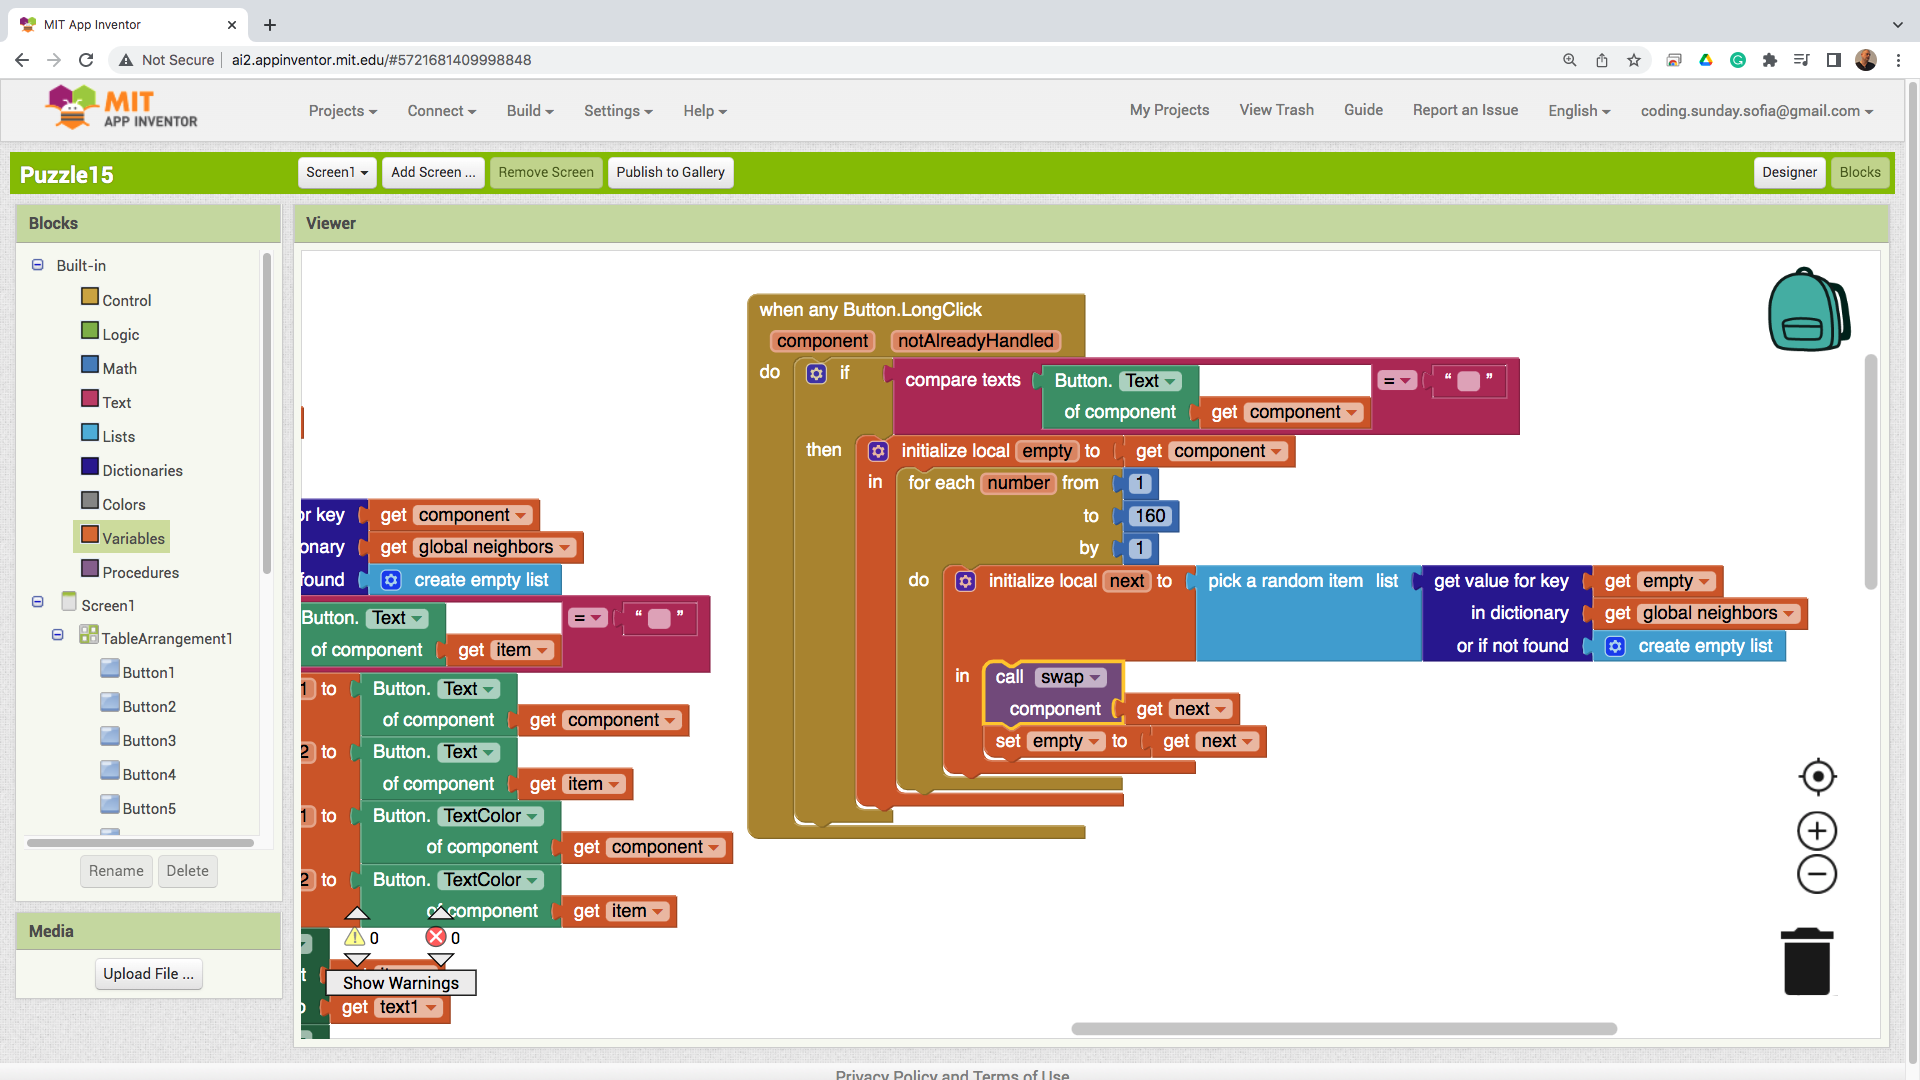
\includegraphics[width=1.0\linewidth,height=0.5\linewidth]{fig060020.png}
  \caption{Размяна на празната клетка}
\label{fig060020}
\end{figure}

След като играта е завършена, проектът може да се публикува за широката аудитория с помощта на бутона „Publish to Gallery“ (Фиг. \ref{fig060021}).

\begin{figure}[H]
  \centering
  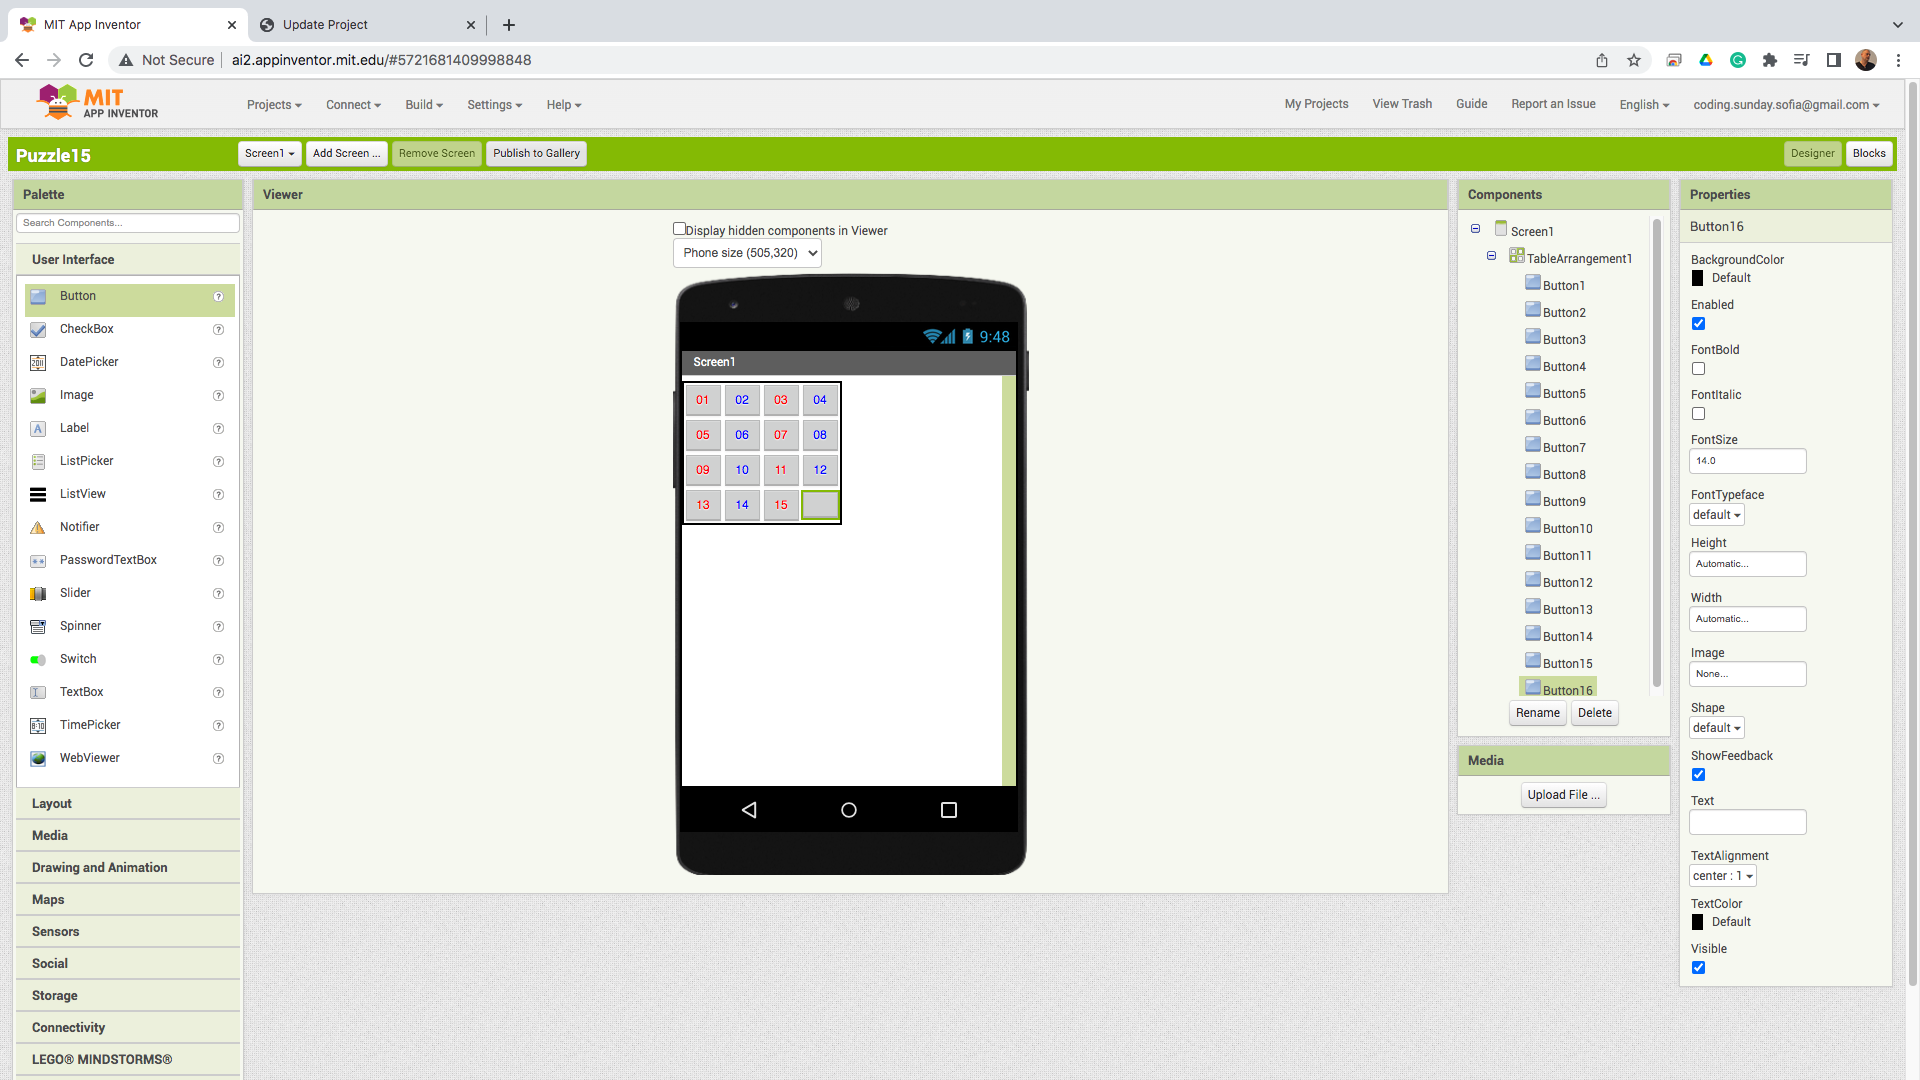
\includegraphics[width=1.0\linewidth,height=0.5\linewidth]{fig060021.png}
  \caption{Бутон за публикуване в галерия}
\label{fig060021}
\end{figure}

Дори семпло описание (Фиг. \ref{fig060022}) на приложението е важно за потребителите, тъй като това е второто нещо, което привлича вниманието им.

\begin{figure}[H]
  \centering
  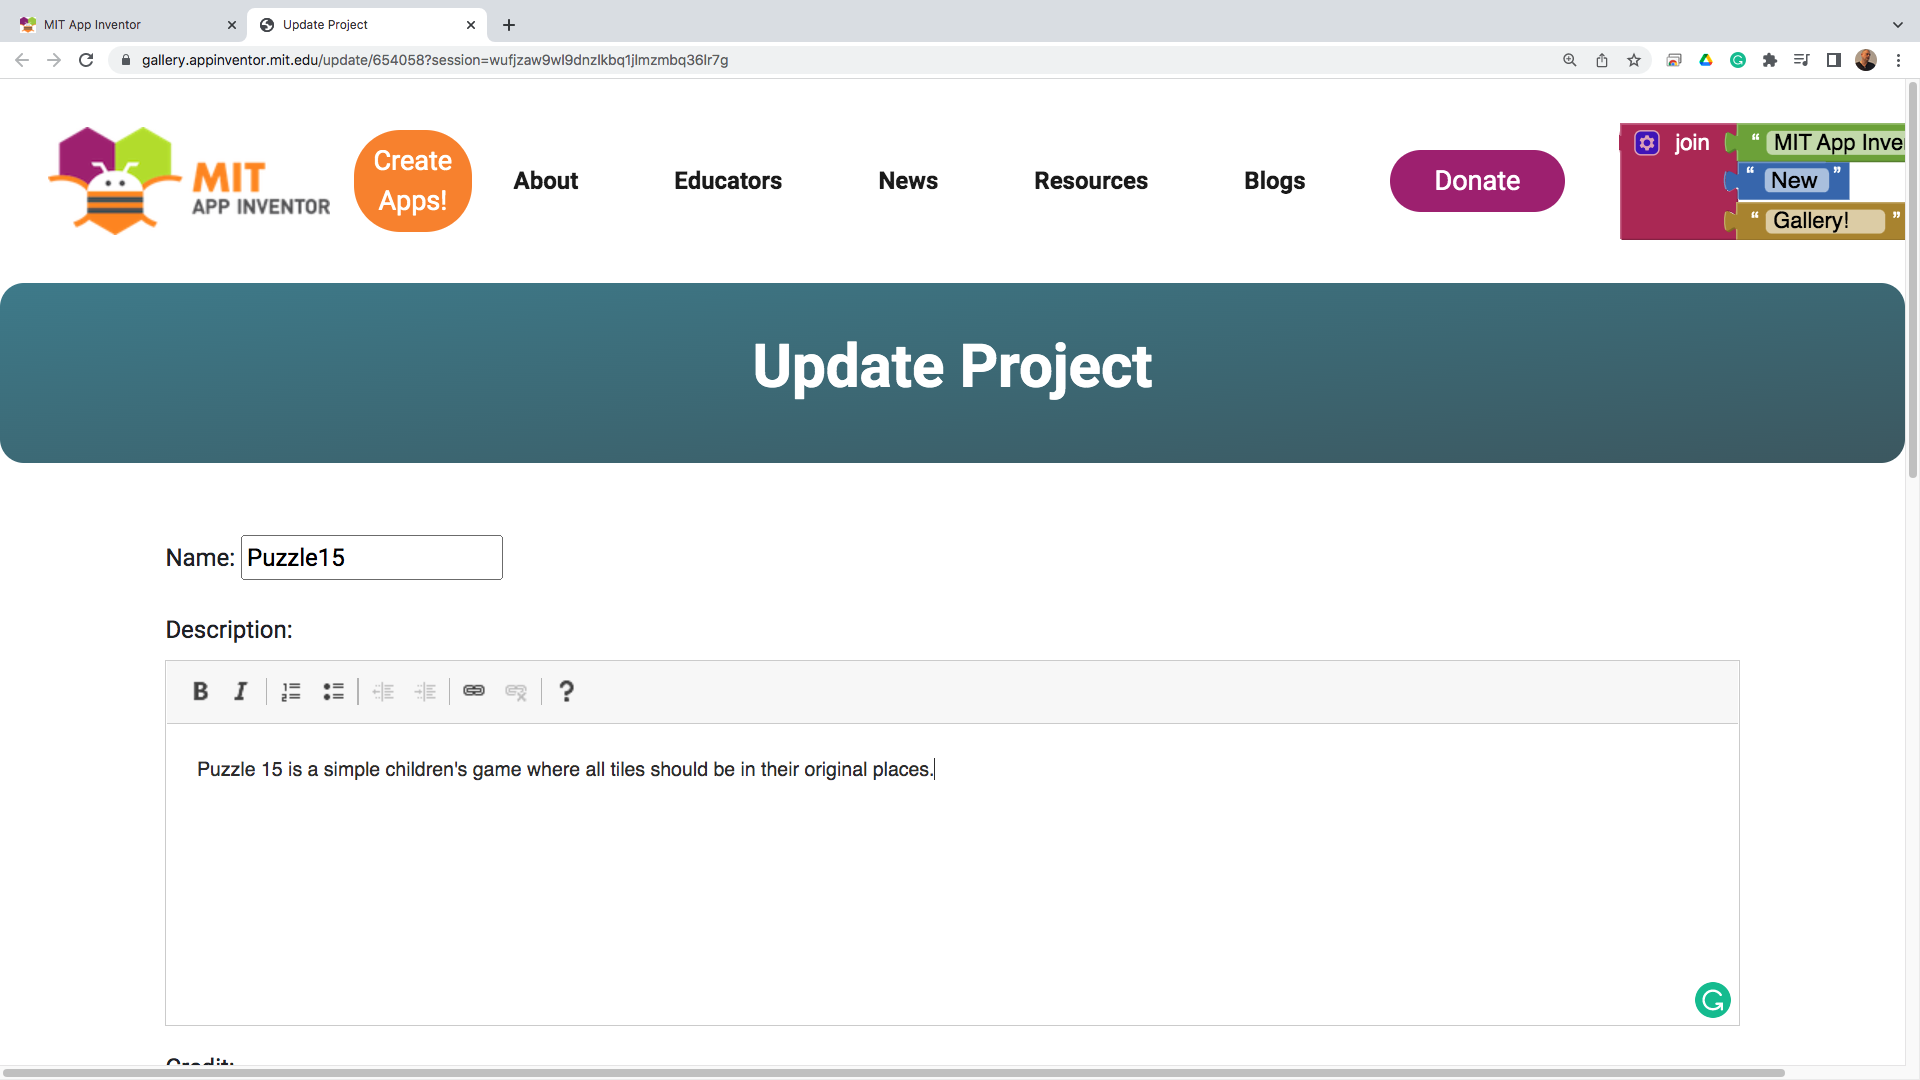
\includegraphics[width=1.0\linewidth,height=0.5\linewidth]{fig060022.png}
  \caption{Описание на приложението}
\label{fig060022}
\end{figure}

Първото най-важно нещо в едно софтуерно приложение е картинка, която най-много може да привлече вниманието на потребителите (Фиг. \ref{fig060023}).

\begin{figure}[H]
  \centering
  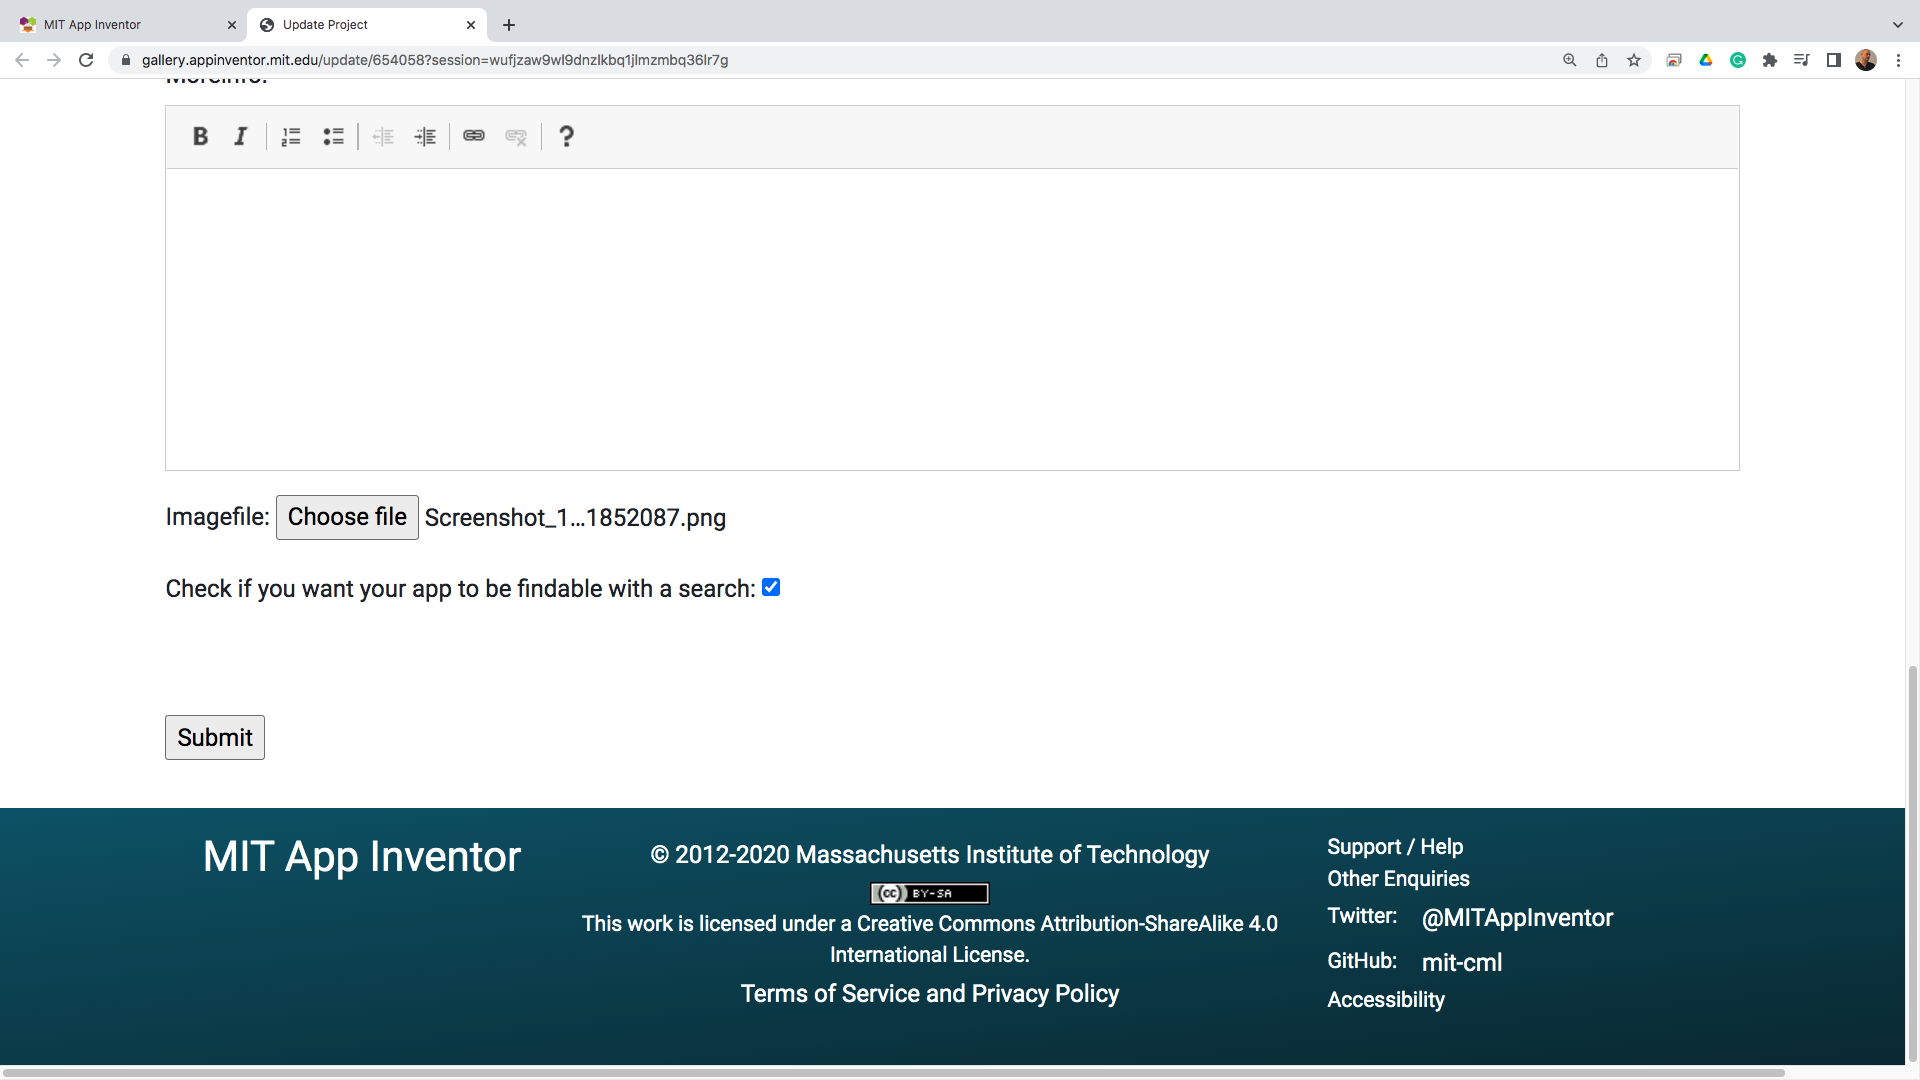
\includegraphics[width=1.0\linewidth,height=0.5\linewidth]{fig060023.png}
  \caption{Картинка за представяне на приложението}
\label{fig060023}
\end{figure}

В публичната страница на проекта (Фиг. \ref{fig060024}), потребителите могат да стартират програмата или да я заредят в средата на App Inventor.

\begin{figure}[H]
  \centering
  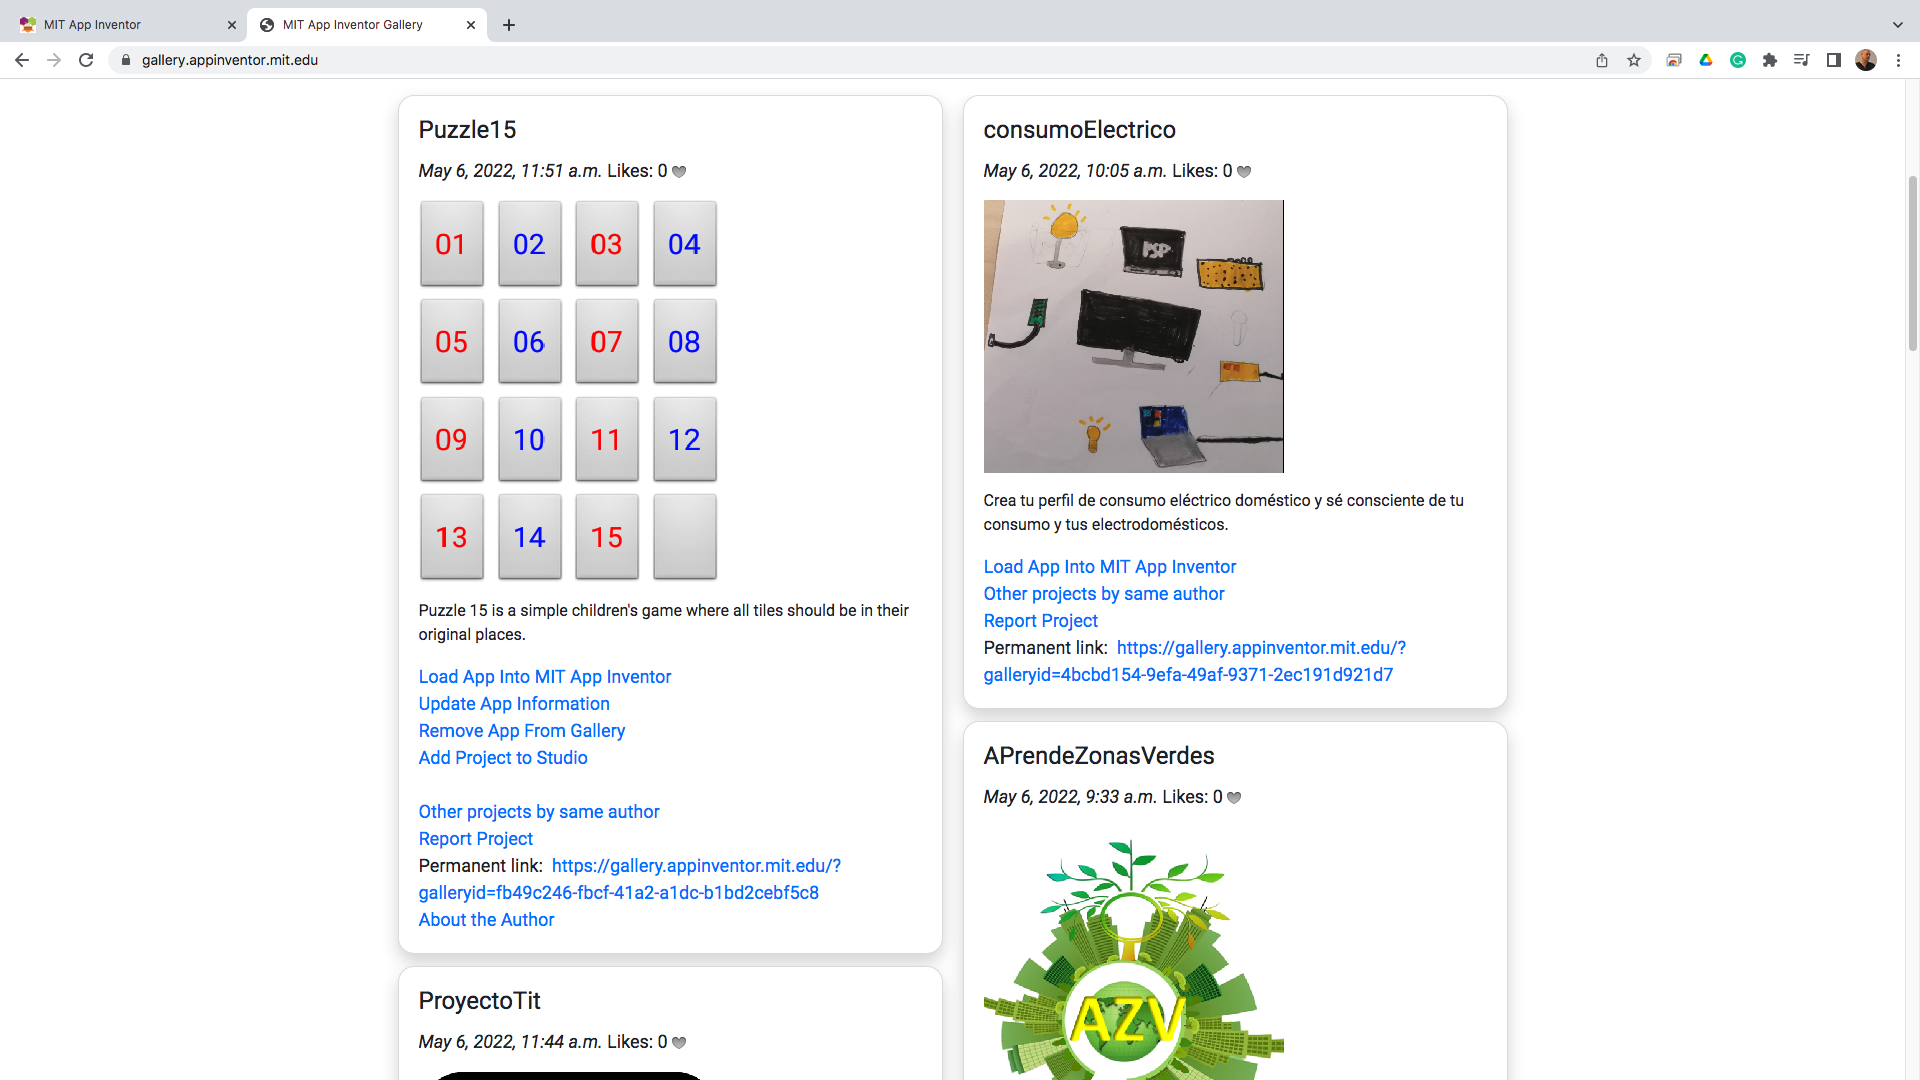
\includegraphics[width=1.0\linewidth,height=0.5\linewidth]{fig060024.png}
  \caption{Публична страница на проета}
\label{fig060024}
\end{figure}

